\documentclass[]{article}
\usepackage{lmodern}
\usepackage{amssymb,amsmath}
\usepackage{ifxetex,ifluatex}
\usepackage{fixltx2e} % provides \textsubscript
\ifnum 0\ifxetex 1\fi\ifluatex 1\fi=0 % if pdftex
  \usepackage[T1]{fontenc}
  \usepackage[utf8]{inputenc}
\else % if luatex or xelatex
  \ifxetex
    \usepackage{mathspec}
  \else
    \usepackage{fontspec}
  \fi
  \defaultfontfeatures{Ligatures=TeX,Scale=MatchLowercase}
\fi
% use upquote if available, for straight quotes in verbatim environments
\IfFileExists{upquote.sty}{\usepackage{upquote}}{}
% use microtype if available
\IfFileExists{microtype.sty}{%
\usepackage{microtype}
\UseMicrotypeSet[protrusion]{basicmath} % disable protrusion for tt fonts
}{}
\usepackage[margin=1in]{geometry}
\usepackage{hyperref}
\hypersetup{unicode=true,
            pdftitle={Machine Learning and AI - Daily and sports activities sensor data},
            pdfauthor={Premysl Velek, 16213669},
            pdfborder={0 0 0},
            breaklinks=true}
\urlstyle{same}  % don't use monospace font for urls
\usepackage{color}
\usepackage{fancyvrb}
\newcommand{\VerbBar}{|}
\newcommand{\VERB}{\Verb[commandchars=\\\{\}]}
\DefineVerbatimEnvironment{Highlighting}{Verbatim}{commandchars=\\\{\}}
% Add ',fontsize=\small' for more characters per line
\usepackage{framed}
\definecolor{shadecolor}{RGB}{248,248,248}
\newenvironment{Shaded}{\begin{snugshade}}{\end{snugshade}}
\newcommand{\AlertTok}[1]{\textcolor[rgb]{0.94,0.16,0.16}{#1}}
\newcommand{\AnnotationTok}[1]{\textcolor[rgb]{0.56,0.35,0.01}{\textbf{\textit{#1}}}}
\newcommand{\AttributeTok}[1]{\textcolor[rgb]{0.77,0.63,0.00}{#1}}
\newcommand{\BaseNTok}[1]{\textcolor[rgb]{0.00,0.00,0.81}{#1}}
\newcommand{\BuiltInTok}[1]{#1}
\newcommand{\CharTok}[1]{\textcolor[rgb]{0.31,0.60,0.02}{#1}}
\newcommand{\CommentTok}[1]{\textcolor[rgb]{0.56,0.35,0.01}{\textit{#1}}}
\newcommand{\CommentVarTok}[1]{\textcolor[rgb]{0.56,0.35,0.01}{\textbf{\textit{#1}}}}
\newcommand{\ConstantTok}[1]{\textcolor[rgb]{0.00,0.00,0.00}{#1}}
\newcommand{\ControlFlowTok}[1]{\textcolor[rgb]{0.13,0.29,0.53}{\textbf{#1}}}
\newcommand{\DataTypeTok}[1]{\textcolor[rgb]{0.13,0.29,0.53}{#1}}
\newcommand{\DecValTok}[1]{\textcolor[rgb]{0.00,0.00,0.81}{#1}}
\newcommand{\DocumentationTok}[1]{\textcolor[rgb]{0.56,0.35,0.01}{\textbf{\textit{#1}}}}
\newcommand{\ErrorTok}[1]{\textcolor[rgb]{0.64,0.00,0.00}{\textbf{#1}}}
\newcommand{\ExtensionTok}[1]{#1}
\newcommand{\FloatTok}[1]{\textcolor[rgb]{0.00,0.00,0.81}{#1}}
\newcommand{\FunctionTok}[1]{\textcolor[rgb]{0.00,0.00,0.00}{#1}}
\newcommand{\ImportTok}[1]{#1}
\newcommand{\InformationTok}[1]{\textcolor[rgb]{0.56,0.35,0.01}{\textbf{\textit{#1}}}}
\newcommand{\KeywordTok}[1]{\textcolor[rgb]{0.13,0.29,0.53}{\textbf{#1}}}
\newcommand{\NormalTok}[1]{#1}
\newcommand{\OperatorTok}[1]{\textcolor[rgb]{0.81,0.36,0.00}{\textbf{#1}}}
\newcommand{\OtherTok}[1]{\textcolor[rgb]{0.56,0.35,0.01}{#1}}
\newcommand{\PreprocessorTok}[1]{\textcolor[rgb]{0.56,0.35,0.01}{\textit{#1}}}
\newcommand{\RegionMarkerTok}[1]{#1}
\newcommand{\SpecialCharTok}[1]{\textcolor[rgb]{0.00,0.00,0.00}{#1}}
\newcommand{\SpecialStringTok}[1]{\textcolor[rgb]{0.31,0.60,0.02}{#1}}
\newcommand{\StringTok}[1]{\textcolor[rgb]{0.31,0.60,0.02}{#1}}
\newcommand{\VariableTok}[1]{\textcolor[rgb]{0.00,0.00,0.00}{#1}}
\newcommand{\VerbatimStringTok}[1]{\textcolor[rgb]{0.31,0.60,0.02}{#1}}
\newcommand{\WarningTok}[1]{\textcolor[rgb]{0.56,0.35,0.01}{\textbf{\textit{#1}}}}
\usepackage{longtable,booktabs}
\usepackage{graphicx,grffile}
\makeatletter
\def\maxwidth{\ifdim\Gin@nat@width>\linewidth\linewidth\else\Gin@nat@width\fi}
\def\maxheight{\ifdim\Gin@nat@height>\textheight\textheight\else\Gin@nat@height\fi}
\makeatother
% Scale images if necessary, so that they will not overflow the page
% margins by default, and it is still possible to overwrite the defaults
% using explicit options in \includegraphics[width, height, ...]{}
\setkeys{Gin}{width=\maxwidth,height=\maxheight,keepaspectratio}
\IfFileExists{parskip.sty}{%
\usepackage{parskip}
}{% else
\setlength{\parindent}{0pt}
\setlength{\parskip}{6pt plus 2pt minus 1pt}
}
\setlength{\emergencystretch}{3em}  % prevent overfull lines
\providecommand{\tightlist}{%
  \setlength{\itemsep}{0pt}\setlength{\parskip}{0pt}}
\setcounter{secnumdepth}{0}
% Redefines (sub)paragraphs to behave more like sections
\ifx\paragraph\undefined\else
\let\oldparagraph\paragraph
\renewcommand{\paragraph}[1]{\oldparagraph{#1}\mbox{}}
\fi
\ifx\subparagraph\undefined\else
\let\oldsubparagraph\subparagraph
\renewcommand{\subparagraph}[1]{\oldsubparagraph{#1}\mbox{}}
\fi

%%% Use protect on footnotes to avoid problems with footnotes in titles
\let\rmarkdownfootnote\footnote%
\def\footnote{\protect\rmarkdownfootnote}

%%% Change title format to be more compact
\usepackage{titling}

% Create subtitle command for use in maketitle
\providecommand{\subtitle}[1]{
  \posttitle{
    \begin{center}\large#1\end{center}
    }
}

\setlength{\droptitle}{-2em}

  \title{Machine Learning and AI - Daily and sports activities sensor data}
    \pretitle{\vspace{\droptitle}\centering\huge}
  \posttitle{\par}
    \author{Premysl Velek, 16213669}
    \preauthor{\centering\large\emph}
  \postauthor{\par}
    \date{}
    \predate{}\postdate{}
  
\usepackage{float}
\usepackage{booktabs}
\usepackage{longtable}
\usepackage{array}
\usepackage{multirow}
\usepackage{wrapfig}
\usepackage{colortbl}
\usepackage{pdflscape}
\usepackage{tabu}
\usepackage{threeparttable}
\usepackage{threeparttablex}
\usepackage[normalem]{ulem}
\usepackage{makecell}
\usepackage{xcolor}

\usepackage{bbm}
\usepackage{graphicx}
\usepackage{float}
\usepackage{breqn}
\usepackage{amsmath}
\usepackage{relsize}
\floatplacement{figure}{H}

\begin{document}
\maketitle

\textbf{Abstract:} This report present a deep neural network to classify
daily and sports activities from motion sensor measurements. A four
stage hyperparameter tuning process was implemented to select the
optimal data pre-processing method, network architecture and
regularization methods. The final model selected has two hidden layers
with 384 units (256-128), early stopping, weight decay
(\(\lambda = 0.0001\)) and dropout (\(rate = 0.2\)) regularization, low
learning rate (0.0005) and batch size of 76 (1 \% of the training
sample). It achieved accuracy of 0.9855 on test data. Following the
tuning process, the impact of the different hyperparameters on the model
performance is discussed.

\hypertarget{introduction}{%
\subsection{Introduction}\label{introduction}}

This report presents the implementation of a deep neural network model
to classify daily and sports activities from motion sensor measurements.
To main goal of the following analysis is to train and test a deep
neural network classification model, present the model configuration and
discuss how it affects the performance of the model.

The resulting model can have various uses, predominantly as part of
mobile apps and wearable devices that follow and track physical
activities of their users (eg. fitness trackers, life-style apps or
personal analytics apps). An important use of the model is within the
rapidly developing field of health data analytics. The model can give
medical doctors detailed information about their patients' physical
activities which can then be coupled with their clinical data and used
to better understand how peoples' life-style affects their
health.\footnote{For overview of the topic see: Loncar-Turukalo T,
  Zdravevski E, Machado da Silva J et al, Literature on Wearable
  Technology for Connected Health: Scoping Review of Research Trends,
  Advances, and Barriers, J Med Internet Res. 2019 Sep 5;21(9):e14017.
  doi: 10.2196/14017.}

\hypertarget{data}{%
\subsection{Data}\label{data}}

The data used to train and test the model are motion sensor measurements
of 19 daily and sports activities, each performed by 8 subjects (4
female, 4 male, between the age of 20 and 30) in their own style for 5
minutes. Each participant in the experiment was equipped with five units
- each with 9 individual sensors - which recorded the movement on the
torso, arms, and legs.

The 19 daily activities performed are:

\begin{itemize}
\tightlist
\item
  Sitting
\item
  Standing
\item
  Lying on back
\item
  Lying on right side
\item
  Ascending stairs
\item
  Descending stairs
\item
  Standing in an elevator still
\item
  Moving around in an elevator
\item
  Walking in a parking lot
\item
  Walking on a flat treadmill with a speed of 4 km/h
\item
  Walking on a 15 deg inclined treadmill with a speed of 4 km/h\\
\item
  Running on a treadmill with a speed of 8 km/h
\item
  Exercising on a stepper
\item
  Exercising on a cross trainer
\item
  Cycling on an exercise bike in horizontal position
\item
  Cycling on an exercise bike in vertical position
\item
  Rowing
\item
  Jumping
\item
  Playing basketball
\end{itemize}

The dataset (sensor data) contains the sensor measurements divided into
5-second signal segments. There is a total of 480 signal segments (60
signal segments for each of the 8 participants) for each activity. These
480 segments are classified into 19 classes corresponding to the daily
and physical activities listed above (total of 9120 segments). Each
signal segment is represented by a 125 × 45 matrix, where rows contain
the 125 samples of data acquired from one of the sensors of one of the
units over a period of 5 seconds, and columns represent the 45
individual sensors (grouped into 5 units).

The dataset was first presented by Altun, Barshan and Tunçel in
2010\footnote{K. Altun, B. Barshan, and O. Tunçel, Comparative study on
  classifying human activities with miniature inertial and magnetic
  sensors, Pattern Recognition, 43(10):3605-3620, October 2010.} and is
available online in the UCI Machine Learning Repository\footnote{\url{https://archive.ics.uci.edu/ml/datasets/Daily+and+Sports+Activities}}.

The dataset is extremely wide, with 5625 (125 x 45) separate variables
for each observation. To visualize the data and explore the
(approximate) relations between the different classes, a principal
component analysis was performed on part of the data (1520
observations). Figure 1 shows the 2d projection of the first two
principal components, amounting to over 32 \% of the variance.

\begin{figure}

{\centering \includegraphics[width=0.8\linewidth]{pca-2} 

}

\caption{Visualisation of part of the sensor data: first two principal components}\label{fig:unnamed-chunk-1}
\end{figure}

To train, validate and test the model, the sensor data was divided into
train, validation and test subsets. The train dataset included 7600
observations (\textasciitilde{} 83.3 \%), the test and validation
dataset contained each 760 observations (\textasciitilde{} 8.3 \%). The
classes were distributed equally in the training set (each class is
represented by 400 observations). The validation and test datasets
combined contained 80 observations for each class; a random split was
used to generate the validation and test datasets which produced a
roughly equal number of classes in each set: the mean number of
observations in the test and validation data for each class was 40, the
standard deviation was 4.73.

\hypertarget{method}{%
\subsection{Method}\label{method}}

The following hyperparameters and configurations were considered during
the training and validation step:

\begin{itemize}
\tightlist
\item
  Data preprocessing
\item
  Model architecture: number of layers and number of nodes in each layer
\item
  Dropout rate
\item
  Weight decay rate
\item
  Batch size
\item
  Learning rate
\item
  Patience rate for early stopping
\end{itemize}

The Adam optimization algorithm and the ReLU activation fictions were
chosen for all models considered. The Adam algorithm is based on
adaptive estimates of lower-order moments (Adaptive moment estimation)
and has been shown to perform better than other stochastic optimization
methods.\footnote{Kingma, DP, Ba J, Adam: A Method for Stochastic
  Optimization, published as a conference paper at the 3rd International
  Conference for Learning Representations, San Diego, 2015, arXiv
  e-prints December 2015, \url{https://arxiv.org/abs/1412.6980}} ReLU
(Rectified Linear Unit) is the most successful and effectively the
default activation function in deep learning models across domains and
research communities.\footnote{Ramachandran P, Zoph B, Le QV, Searching
  for Activation Functions, arXiv e-prints October 2017,
  \url{https://arxiv.org/abs/1710.05941v2}}

To identify the optimal model configuration, several models with
different parameters were considered in four successive stages: (1)
Pre-rocessing, (2)architecture, (3) Elimination tuning and (4) Final
tuning.

Each model was trained on the training data and validated using the
validation set. All model were trained over a maximum of 100 epochs, the
performance on both train and validation set was measured after each
epoch, using the accuracy metric (proportion of correctly classified
classes to all classes). In Stages 3 and 4, each model considered was
also evaluated using the test data.

The final performance on the validation and test data, and the shape of
the learning curve were used to select the optimal hyperparamenters
setting. The accuracy performance of the final selected model on test
data was reported as the main performance metric.

The model was implemented using the R interface of the Keras
API\footnote{\url{https://keras.rstudio.com/index.html}}.

\hypertarget{stage-1-data-preprocessing}{%
\subsubsection{Stage 1: Data
preprocessing}\label{stage-1-data-preprocessing}}

To select the optimal method of data preprocessing, three methods were
tested: (1) Normalization, (2) Standardization, and (3) Identity (the
original raw measurements).

The data obtained by the three preprocessing method were fitted to the
same simple neural network model, with 2 layers and 512-128 nodes, ReLU
activation function, softmax output activation function and Adam
optimizer with the learning rate of 0.001. Figure 2 shows the training
and validation learning curves for the three processing methods.

\begin{figure}

{\centering \includegraphics[width=0.8\linewidth]{pre-process-2} 

}

\caption{Training and validation performance for models fitted to normalised, standardised and raw data}\label{fig:unnamed-chunk-2}
\end{figure}

Based on the result of the training and validation data, the
standardization method was selected for the final model. The model with
standardization data had the best training and validation performance
and relatively steady learning curve as compared to the two other
methods. It also better generalized on validation data as compared to
the normalized dataset which had similar training accuracy but lower
validation accuracy.

\hypertarget{stage-2-architecture}{%
\subsubsection{Stage 2: Architecture}\label{stage-2-architecture}}

To identify the optimal number of hidden layers, three different models
with 2, 4 and 6 layers were trained and validated, using a simple model
with ReLU activation function, softmax output activation function and
Adam optimizer. The number of layers in the models were as follows:

\begin{itemize}
\tightlist
\item
  2-layer model: 512-256
\item
  4-layer model: 512-256-128-64
\item
  6-layer model: 512-256-192-128-64-32
\end{itemize}

Figure 3 shows the training and validation learning curves for the three
models. It's clear that the number of layers doesn't have a significant
impact on the performance of the model, and more layers don't improve
the performance of the model - the final accuracy values for all three
models are within a narrow range. Even though the performance of the
6-layer model was more stable throughout the training epoch, this is not
a sufficient reason to decide for more complex model, as regularization
was addressed only in the stages 3 and 4.

\begin{figure}

{\centering \includegraphics[width=0.7\linewidth]{layers-2} 

}

\caption{Training and validation performance for models with different number of layers}\label{fig:unnamed-chunk-3}
\end{figure}

As simpler models should be preferred, a 2-layer model was selected at
this stage.

\hypertarget{stage-3-elimination-tuning}{%
\paragraph{Stage 3: Elimination
tuning}\label{stage-3-elimination-tuning}}

Following the selection of data preprocessing method and the number of
layers, all remaining hyperparameters were selected using a random grid
search.\footnote{The tfruns package was used to manage the training runs
  during the tuning process,
  \url{https://cran.r-project.org/package=tfruns}} Grid search
systematically searches through the configuration space and can fit
model with every possible configurations, given the number of parameters
we want to tune and the range of possible values.

In Stage 3 a wider set of values was considered with the aim to narrow
down the range of possible values. Rather than identify the best
hyperparameters for the model, the goal was to identify values or range
of values for that don't produce good results. Those values were
subsequently eliminated from the grid search implemented in Stage 4.

In the Elimination tuning, the following values were considered:

\begin{longtable}[]{@{}ll@{}}
\toprule
\endhead
dropout & 0, 0.2, 0.4\tabularnewline
nodes\_1 & 512, 256\tabularnewline
nodes\_2 & 256, 128, 64\tabularnewline
lambda & 0, 0.0001, 0.0015, 0.018\tabularnewline
batch\_size & 22, 76, 152\tabularnewline
learning\_rate & 0.001, 0.005, 0.01\tabularnewline
patience & 10, 20\tabularnewline
\bottomrule
\end{longtable}

There is 1296 possible combinations of the hyperparameters. The random
grid search selected randomly 38 (3 \%) of the possible combinations,
and recorded the training, validation and test metrics for each of them.
Figure 4 shows the validation learning curves of those 38 models in a
series of plots to visualize how the different hyperparameters impact
the validation results.\footnote{The effect of batch size is not
  included}

\begin{figure}

{\centering \includegraphics[width=0.8\linewidth]{eliminace} 

}

\caption{Figure 4: Validation performance for 38 models with different hyperparameters}\label{fig:unnamed-chunk-5}
\end{figure}

The 10 worst performing models are listed in the table below:

\begin{table}[H]
\centering
\begin{tabular}{l|r|r|r|r|r|r|r}
\hline
  & dropout & nodes\_1 & nodes\_2 & lambda & batch & lr & patience\\
\hline
23 & 0.4 & 512 & 256 & 0.0001 & 22 & 0.010 & 20\\
\hline
24 & 0.2 & 512 & 64 & 0.0015 & 22 & 0.010 & 20\\
\hline
16 & 0.2 & 512 & 128 & 0.0001 & 76 & 0.010 & 20\\
\hline
37 & 0.0 & 256 & 128 & 0.0001 & 22 & 0.010 & 20\\
\hline
4 & 0.4 & 256 & 128 & 0.0183 & 22 & 0.010 & 10\\
\hline
13 & 0.0 & 256 & 64 & 0.0001 & 22 & 0.010 & 20\\
\hline
3 & 0.2 & 512 & 128 & 0.0001 & 22 & 0.005 & 20\\
\hline
35 & 0.0 & 512 & 256 & 0.0000 & 76 & 0.010 & 20\\
\hline
33 & 0.2 & 256 & 64 & 0.0015 & 76 & 0.010 & 20\\
\hline
31 & 0.2 & 256 & 64 & 0.0015 & 76 & 0.010 & 10\\
\hline
\end{tabular}
\end{table}

Based on the results of the first grid search, the following
hyperparameters negatively impacted the model performance and were
eliminated from the tuning grid in the Stage 4.

\begin{enumerate}
\def\labelenumi{\arabic{enumi}.}
\tightlist
\item
  Learning rate of 0.01 and 0.005
\item
  Lambda values of 0.0183 and 0.0015
\item
  The number of units 512 in the first hidden layer
\item
  The number of units 64 and 256 in the second hidden layer
\end{enumerate}

As the results of the Stage 3 showed that low learning rates were much
better choice for the model, an extra value of 0.0005 for learning rate
was added to the grid.

On the contrary, there was no clear evidence that the different values
for the dropout rate and for batch size significantly affect the model:
the models with different dropout rate and batch size scored both low
and high. While batch sizes of 22 and 76 produced the worst performing
models (see the table above), they were also included in one of the best
models. All values considered for dropout rate were equally represented
among best and worst performing models. This could be because those two
hyperparameters in reality don't affect significantly the model or
because of the limited scope of the grid search (3 \% of the possible
combinations)\footnote{There were only eight models with dropout rate
  0.4, five of them coupled with learning rate of 0.01 and 0.005, which
  we excluded already from the grid. So there were not enough models
  trained that would conclusively show whether or not dropout rate of
  0.4 positively affect the performance.}

As for the patience values, the learning curves of the high scoring
models didn't show significant signs of declining performance over the
epochs. This means that that we could keep the patience values higher
without worrying about declining performance. In the next stage, only
the patience value of 20 was considered.

All values of dropout rate and batch size were kept in the grid search
in the next phase.

\hypertarget{stage-4-final-tuning}{%
\paragraph{Stage 4: Final tuning}\label{stage-4-final-tuning}}

Following the results of the elimination tuning, the range of possible
configuration settings was reduced from 1296 to 48. Using similar
approach and similar model as in Stage 3, the following values were
considered:

\begin{table}[H]
\centering
\begin{tabular}{l|l}
\hline
dropout & 0, 0.2, 0.4\\
\hline
lambda & 0, 1e-04\\
\hline
batch\_size & 22, 76, 152\\
\hline
learning\_rate & 0.0005, 0.001\\
\hline
\end{tabular}
\end{table}

The number of nodes and the patience value were fixed for all models.

At this stage a full grid search was performed, testing the complete
range of possible configurations.

The hyperparameters for the ten best performing models - based on
accuracy on the test data - are listed in the table below:

\begin{table}[H]
\centering
\begin{tabular}{l|r|r|r|r|r|r|r}
\hline
  & test acc & val acc & dropout & lambda & batch & lr & epochs\\
\hline
27 & 0.9868 & 0.9921 & 0.0 & 1e-04 & 76 & 1e-03 & 55\\
\hline
30 & 0.9868 & 0.9855 & 0.0 & 0e+00 & 76 & 1e-03 & 34\\
\hline
8 & 0.9855 & 0.9868 & 0.2 & 1e-04 & 76 & 5e-04 & 78\\
\hline
6 & 0.9842 & 0.9803 & 0.0 & 0e+00 & 152 & 5e-04 & 37\\
\hline
1 & 0.9829 & 0.9737 & 0.4 & 1e-04 & 152 & 5e-04 & 50\\
\hline
11 & 0.9829 & 0.9842 & 0.2 & 0e+00 & 76 & 5e-04 & 48\\
\hline
13 & 0.9829 & 0.9816 & 0.4 & 1e-04 & 22 & 5e-04 & 99\\
\hline
24 & 0.9829 & 0.9868 & 0.0 & 0e+00 & 152 & 1e-03 & 35\\
\hline
32 & 0.9829 & 0.9750 & 0.2 & 1e-04 & 22 & 1e-03 & 51\\
\hline
16 & 0.9816 & 0.9763 & 0.4 & 0e+00 & 22 & 5e-04 & 73\\
\hline
\end{tabular}
\end{table}

We see that these best performing models have the accuracy on the test
data over 0.98. Figure 5 show the learning curves for validation
accuracy (left) and validation loss (right) for all models with the 10
best performing models highlighted:

\begin{figure}

{\centering 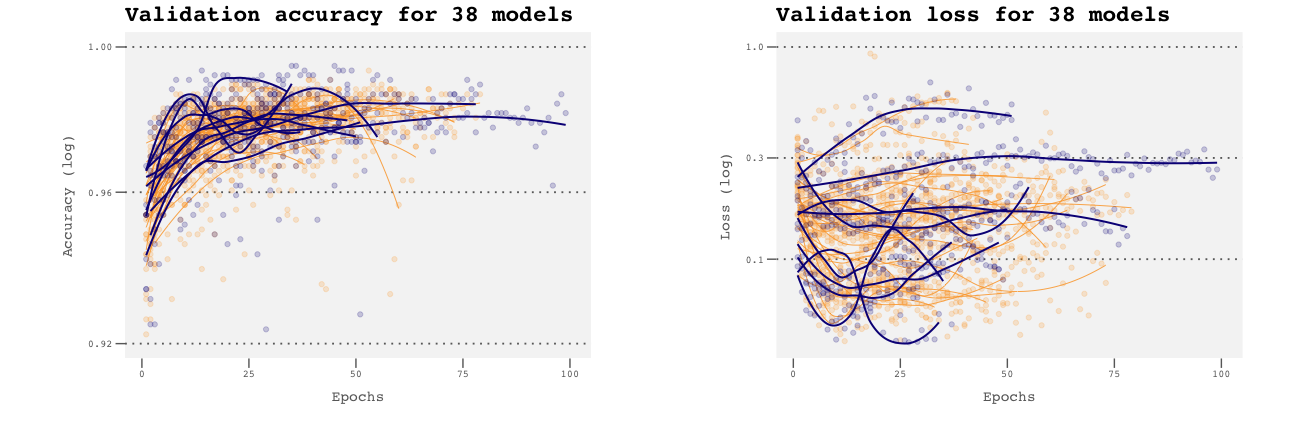
\includegraphics[width=1\linewidth]{val-loss} 

}

\caption{Validation accuracy and loss for 38 models with different hyperparameters}\label{fig:unnamed-chunk-9}
\end{figure}

The learning curves suggest that many of the best performing models are
over-fitted. Although their accuracy is high, the validation loss are
either increasing or unstable. The final model was selected based on the
test accuracy, test loss and a visual inspection of the learning curves
of the best models.

\hypertarget{results-and-discussion}{%
\subsubsection{Results and discussion}\label{results-and-discussion}}

The final model selected as a result of four-stage training process has
the following configuration and hyperparameters:

\begin{itemize}
\tightlist
\item
  Two hidden layers with 256-128 nodes
\item
  Activation function: ReLU
\item
  Output activation function: Softmax
\item
  Optimization method: Adam
\item
  Weight decay regularization rate (lambda): 0.0001
\item
  Dropout regularization rate: 0.2
\item
  Early stopping regularization (patience): 20
\item
  Batch size: 76
\item
  Learning rate: 0.0005
\end{itemize}

The accuracy on the test data for this model is 0.9855 (the third best
accuracy score). Overall, the hyperparameter tuning process showed that
there are several possible configurations for the model. Of the 38
models considered in the final stage, 15 reached test accuracy of over
0.98.

Figure 6 shows the accuracy training and validation curve for the final
model:

\begin{figure}

{\centering 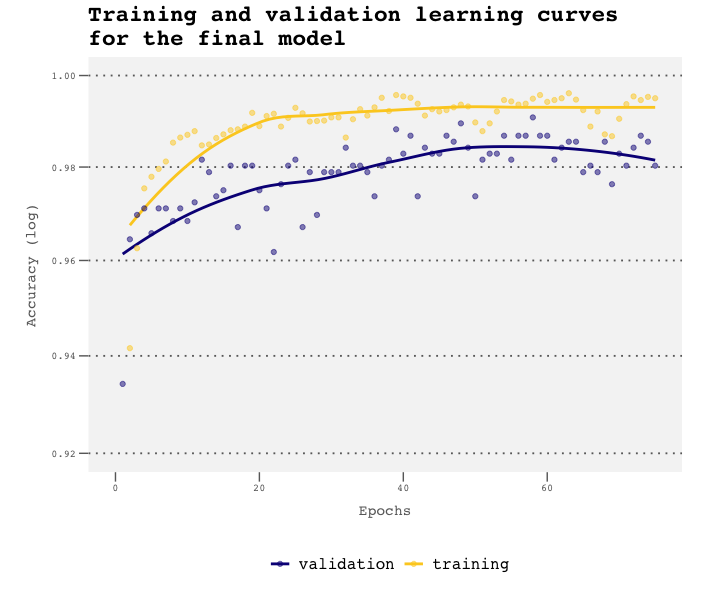
\includegraphics[width=0.8\linewidth]{final-2a} 

}

\caption{Training and validation accuracy learning curve for the final models}\label{fig:unnamed-chunk-10}
\end{figure}

The learning rate seems to have the biggest impact on the model
performance, whereby models with learning rate of 0.001 or lower clearly
outperform models with higher learning rates. Similarly, higher values
of lambda for weight decay regularization produced sub-optimal
solutions. The best models have the value of lambda either zero or close
to zero (0.0001).

Dropout regularization method doesn't have strong influence on the
model, as the results show that models with high test accuracy have
their dropout rate ranging from 0 to 0.4. Similarly, batch size don't
significantly impact the model performance as models with all three
values (22, 76, 152) produce models good model (with accuracy score of
over 0.98).

The result also show that most models converge to their optimal
performance very early on in training process. After around 30 epochs
the increase in performance is minimal. In most cases the early stopping
regularization stopped the training process within the first 50 epochs.
No model completed the maximum of 100 epochs, only one model reached
over 90 epochs, additional four models (including the final selected
model) reached more than 70 training epochs. The optimal number of epoch
is likely around 60 epochs. After this, most model become over-fitted
with corresponding decrease in accuracy and increase in the loss
function.

In terms of the model architecture, the results presented indicate that
higher number of hidden layers and higher number of nodes don't increase
the performance of the model.

\hypertarget{conclusion}{%
\subsubsection{Conclusion}\label{conclusion}}

This report presented an implementation of deep neural network to
classify daily and sporting activities based on motion sensor
measurement. The final test accuracy reached over 0.98 \%. Considering
the intended use of the model (healthy life-style or heath care), this
accuracy is sufficient for effective prediction of daily physical
activities.

\hypertarget{references}{%
\subsubsection{References}\label{references}}

\begin{itemize}
\item
  R Core Team (2013). R: A language and environment for statistical
  computing. R Foundation for Statistical Computing, Vienna, Austria.
  \url{http://www.R-project.org/}.
\item
  R interface of the Keras API,
  \url{https://keras.rstudio.com/index.html}
\item
  tfruns R package: \url{https://cran.r-project.org/package=tfruns}
\item
  gglot2 R package: Wickham H (2016). ggplot2: Elegant Graphics for Data
  Analysis. Springer-Verlag New York. ISBN 978-3-319-24277-4,
  \url{https://ggplot2.tidyverse.org}.
\item
  viridis R package, \url{https://CRAN.R-project.org/package=viridis}
\item
  Kingma, DP, Ba J, Adam: A Method for Stochastic Optimization,
  published as a conference paper at the 3rd International Conference
  for Learning Representations, San Diego, 2015, arXiv e-prints December
  2015, \url{https://arxiv.org/abs/1412.6980}
\item
  Ramachandran P, Zoph B, Le QV, Searching for Activation Functions,
  arXiv e-prints October 2017, \url{https://arxiv.org/abs/1710.05941v2}
\item
  K. Altun, B. Barshan, and O. Tunçel, Comparative study on classifying
  human activities with miniature inertial and magnetic sensors, Pattern
  Recognition, 43(10):3605-3620, October 2010,
  \url{https://archive.ics.uci.edu/ml/datasets/Daily+and+Sports+Activities}
\item
  Loncar-Turukalo T, Zdravevski E, Machado da Silva J et al, Literature
  on Wearable Technology for Connected Health: Scoping Review of
  Research Trends, Advances, and Barriers, J Med Internet Res. 2019 Sep
  5;21(9):e14017. doi: 10.2196/14017.
\end{itemize}

\hypertarget{appendix-1---r-script}{%
\subsection{Appendix 1 - R script}\label{appendix-1---r-script}}

\begin{Shaded}
\begin{Highlighting}[]
\CommentTok{# libraries}
\KeywordTok{library}\NormalTok{(keras)}
\KeywordTok{library}\NormalTok{(ggplot2)}
\KeywordTok{library}\NormalTok{(reshape2)}
\KeywordTok{library}\NormalTok{(viridis)}
\KeywordTok{library}\NormalTok{(dplyr)}
\KeywordTok{library}\NormalTok{(tfruns)}
\KeywordTok{library}\NormalTok{(gridExtra)}
\KeywordTok{library}\NormalTok{(jsonlite)}


\CommentTok{# load helper functions}
\KeywordTok{source}\NormalTok{(}\StringTok{'helpers.R'}\NormalTok{)}

\CommentTok{# load data}
\KeywordTok{load}\NormalTok{(}\StringTok{'data_activity_recognition.RData'}\NormalTok{)}

\CommentTok{# check the dimensions}
\KeywordTok{dim}\NormalTok{(x_test)}
\KeywordTok{dim}\NormalTok{(x_train)}

\CommentTok{# reshape the matrix into vectors - each signal segment is represented by a }
\CommentTok{# vector of 125*45 measurements}
\NormalTok{x_train <-}\StringTok{ }\KeywordTok{array_reshape}\NormalTok{(x_train, }\KeywordTok{c}\NormalTok{(}\KeywordTok{nrow}\NormalTok{(x_train), }\DecValTok{125} \OperatorTok{*}\StringTok{ }\DecValTok{45}\NormalTok{)) }
\NormalTok{x_test <-}\StringTok{ }\KeywordTok{array_reshape}\NormalTok{(x_test, }\KeywordTok{c}\NormalTok{(}\KeywordTok{nrow}\NormalTok{(x_test), }\DecValTok{125} \OperatorTok{*}\StringTok{ }\DecValTok{45}\NormalTok{))}

\CommentTok{######################################################################################}
\CommentTok{### Visualisation of the classes #####################################################}
\CommentTok{######################################################################################}

\CommentTok{# reduce the dimension of the data with PCA}
\NormalTok{x_test_pca <-}\StringTok{ }\KeywordTok{prcomp}\NormalTok{(x_test)}

\CommentTok{# compute cumulative proportion of variance }
\NormalTok{prop <-}\StringTok{ }\KeywordTok{cumsum}\NormalTok{(x_test_pca}\OperatorTok{$}\NormalTok{sdev}\OperatorTok{^}\DecValTok{2}\NormalTok{) }\OperatorTok{/}\StringTok{ }\KeywordTok{sum}\NormalTok{(x_test_pca}\OperatorTok{$}\NormalTok{sdev}\OperatorTok{^}\DecValTok{2}\NormalTok{) }

\CommentTok{# proportion of variance explained by the first two and ten components}
\NormalTok{prop[}\DecValTok{2}\NormalTok{]}

\CommentTok{# plot the first two principal components (around 31 % of the variance)}
\KeywordTok{ggplot}\NormalTok{(}\KeywordTok{as.data.frame}\NormalTok{(x_test_pca}\OperatorTok{$}\NormalTok{x[, }\KeywordTok{c}\NormalTok{(}\DecValTok{1}\OperatorTok{:}\DecValTok{2}\NormalTok{)]), }\KeywordTok{aes}\NormalTok{(}\DataTypeTok{x =}\NormalTok{ x_test_pca}\OperatorTok{$}\NormalTok{x[, }\DecValTok{1}\NormalTok{], }\DataTypeTok{y =}\NormalTok{ x_test_pca}\OperatorTok{$}\NormalTok{x[, }\DecValTok{2}\NormalTok{])) }\OperatorTok{+}
\StringTok{  }\KeywordTok{geom_point}\NormalTok{(}\KeywordTok{aes}\NormalTok{(}\DataTypeTok{colour =}\NormalTok{ y_test)) }\OperatorTok{+}
\StringTok{  }\KeywordTok{theme_pv}\NormalTok{() }\OperatorTok{+}
\StringTok{  }\KeywordTok{scale_colour_viridis_d}\NormalTok{(}\DataTypeTok{option =} \StringTok{'C'}\NormalTok{, }\DataTypeTok{name =} \StringTok{'Type of activity:'}\NormalTok{) }\OperatorTok{+}
\StringTok{  }\KeywordTok{labs}\NormalTok{(}\DataTypeTok{title =} \StringTok{'Sport activities reduced to }\CharTok{\textbackslash{}n}\StringTok{two dimensions'}\NormalTok{, }\DataTypeTok{y =} \StringTok{"PC2"}\NormalTok{, }\DataTypeTok{x =} \StringTok{"PC1"}\NormalTok{) }\OperatorTok{+}
\StringTok{  }\KeywordTok{theme}\NormalTok{(}\DataTypeTok{legend.position =} \StringTok{'right'}\NormalTok{, }
        \DataTypeTok{legend.text =} \KeywordTok{element_text}\NormalTok{(}\DataTypeTok{size =} \DecValTok{12}\NormalTok{)) }

\CommentTok{#####}

\CommentTok{######## Data preparation ######################################################}

\CommentTok{# see the range of the value}
\KeywordTok{range}\NormalTok{(x_train)}

\CommentTok{# convert classes from character to numeric value}
\NormalTok{y_test <-}\StringTok{ }\KeywordTok{as.factor}\NormalTok{(y_test)}
\NormalTok{y_test <-}\StringTok{ }\KeywordTok{as.numeric}\NormalTok{(y_test)}
\NormalTok{y_test <-}\StringTok{ }\NormalTok{y_test }\OperatorTok{-}\StringTok{ }\DecValTok{1}

\NormalTok{y_train <-}\StringTok{ }\KeywordTok{as.factor}\NormalTok{(y_train)}
\NormalTok{y_train <-}\StringTok{ }\KeywordTok{as.numeric}\NormalTok{(y_train)}
\NormalTok{y_train <-}\StringTok{ }\NormalTok{y_train }\OperatorTok{-}\StringTok{ }\DecValTok{1}

\CommentTok{# one-hot encoding}
\NormalTok{y_train <-}\StringTok{ }\KeywordTok{to_categorical}\NormalTok{(y_train) }
\NormalTok{y_test <-}\StringTok{ }\KeywordTok{to_categorical}\NormalTok{(y_test)}

\CommentTok{######## Validation-test split ######################################################}

\CommentTok{# split the test data in two halves: one for validation}
\CommentTok{# and the other for actual testing}
\KeywordTok{set.seed}\NormalTok{(}\DecValTok{12}\NormalTok{)}

\NormalTok{val <-}\StringTok{ }\KeywordTok{sample}\NormalTok{(}\DecValTok{1}\OperatorTok{:}\KeywordTok{nrow}\NormalTok{(x_test), }\KeywordTok{floor}\NormalTok{(}\KeywordTok{nrow}\NormalTok{(x_test) }\OperatorTok{*}\StringTok{ }\FloatTok{0.5}\NormalTok{)) }
\NormalTok{test <-}\StringTok{ }\KeywordTok{setdiff}\NormalTok{(}\DecValTok{1}\OperatorTok{:}\KeywordTok{nrow}\NormalTok{(x_test), val) }

\NormalTok{x_val <-}\StringTok{ }\NormalTok{x_test[val, ]}
\NormalTok{y_val <-}\StringTok{ }\NormalTok{y_test[val, ]}

\NormalTok{x_test <-}\StringTok{ }\NormalTok{x_test[test, ]}
\NormalTok{y_test <-}\StringTok{ }\NormalTok{y_test[test, ]}

\NormalTok{V <-}\StringTok{ }\KeywordTok{ncol}\NormalTok{(x_train)}
\NormalTok{N <-}\StringTok{ }\KeywordTok{nrow}\NormalTok{(x_train)}

\CommentTok{# check if the classes are distributed equaly in the test and val data}
\KeywordTok{mean}\NormalTok{(}\KeywordTok{colSums}\NormalTok{(y_val))}
\KeywordTok{mean}\NormalTok{(}\KeywordTok{colSums}\NormalTok{(y_test))}

\KeywordTok{sd}\NormalTok{(}\KeywordTok{colSums}\NormalTok{(y_val))}
\KeywordTok{sd}\NormalTok{(}\KeywordTok{colSums}\NormalTok{(y_test))}

\CommentTok{#################################################################################################################}
\CommentTok{################ Selecting data preprocessing methods ###########################################################}
\CommentTok{#################################################################################################################}

\CommentTok{# normalisation}
\NormalTok{normalise <-}\StringTok{ }\ControlFlowTok{function}\NormalTok{(x)\{}
\NormalTok{  (x }\OperatorTok{-}\StringTok{ }\KeywordTok{min}\NormalTok{(x)) }\OperatorTok{/}\StringTok{ }\NormalTok{(}\KeywordTok{max}\NormalTok{(x) }\OperatorTok{-}\StringTok{ }\KeywordTok{min}\NormalTok{(x))}
\NormalTok{\}}

\NormalTok{x_train_n <-}\StringTok{ }\KeywordTok{apply}\NormalTok{(x_train, }\DecValTok{2}\NormalTok{, normalise)}
\NormalTok{x_val_n <-}\StringTok{ }\KeywordTok{apply}\NormalTok{(x_val, }\DecValTok{2}\NormalTok{, normalise)}

\CommentTok{# standardisation}
\NormalTok{x_train_s <-}\StringTok{ }\KeywordTok{scale}\NormalTok{(x_train)}
\NormalTok{x_val_s <-}\StringTok{ }\KeywordTok{scale}\NormalTok{(x_val)}



\CommentTok{# dnn to select the data preprocessing method}
\NormalTok{model <-}\StringTok{ }\KeywordTok{keras_model_sequential}\NormalTok{() }\OperatorTok
\StringTok{  }\KeywordTok{layer_dense}\NormalTok{(}\DataTypeTok{units =} \DecValTok{512}\NormalTok{, }\DataTypeTok{input_shape =}\NormalTok{ V, }\DataTypeTok{activation =} \StringTok{"relu"}\NormalTok{, }\DataTypeTok{name =} \StringTok{"layer_1"}\NormalTok{) }\OperatorTok
\StringTok{  }\KeywordTok{layer_dense}\NormalTok{(}\DataTypeTok{units =} \DecValTok{128}\NormalTok{, }\DataTypeTok{activation =} \StringTok{"relu"}\NormalTok{, }\DataTypeTok{name =} \StringTok{"layer_2"}\NormalTok{) }\OperatorTok
\StringTok{  }\KeywordTok{layer_dense}\NormalTok{(}\DataTypeTok{units =} \KeywordTok{ncol}\NormalTok{(y_train), }\DataTypeTok{activation =} \StringTok{"softmax"}\NormalTok{, }\DataTypeTok{name =} \StringTok{"layer_out"}\NormalTok{) }\OperatorTok
\StringTok{  }
\StringTok{  }\KeywordTok{compile}\NormalTok{(}
    \DataTypeTok{loss =} \StringTok{"categorical_crossentropy"}\NormalTok{, }
    \DataTypeTok{metrics =} \StringTok{"accuracy"}\NormalTok{,}
    \DataTypeTok{optimizer =} \KeywordTok{optimizer_adam}\NormalTok{()}
\NormalTok{  )}

\CommentTok{# put the three data in a list}
\NormalTok{dprep_test <-}\StringTok{ }\KeywordTok{list}\NormalTok{(}\DataTypeTok{norm =} \KeywordTok{list}\NormalTok{(x_train_n, x_val_n),}
                   \DataTypeTok{identity =} \KeywordTok{list}\NormalTok{(x_train, x_val), }
                   \DataTypeTok{stand =} \KeywordTok{list}\NormalTok{(x_train_s, x_val_s))}

\CommentTok{# initialise list to store the learning curve data}
\NormalTok{fits <-}\StringTok{ }\KeywordTok{list}\NormalTok{()}


\CommentTok{# run three models}
\ControlFlowTok{for}\NormalTok{(i }\ControlFlowTok{in} \DecValTok{1}\OperatorTok{:}\DecValTok{3}\NormalTok{)\{}
\NormalTok{  fit <-}\StringTok{ }\NormalTok{model }\OperatorTok\StringTok{ }\KeywordTok{fit}\NormalTok{(}
    \DataTypeTok{x =}\NormalTok{ dprep_test[[i]][}\DecValTok{1}\NormalTok{], }\DataTypeTok{y =}\NormalTok{ y_train,}
    \DataTypeTok{validation_data =} \KeywordTok{list}\NormalTok{(dprep_test[[i]][}\DecValTok{2}\NormalTok{], y_val),}
    \DataTypeTok{epochs =} \DecValTok{100}\NormalTok{,}
    \DataTypeTok{verbose =} \DecValTok{1}\NormalTok{)}
\NormalTok{  fits[[i]] <-}\StringTok{ }\NormalTok{fit}
\NormalTok{\}}


\CommentTok{###### Plotting #############}

\NormalTok{coln <-}\StringTok{ }\KeywordTok{c}\NormalTok{(}\StringTok{'Identity_train'}\NormalTok{, }\StringTok{'Identity_val'}\NormalTok{,}
          \StringTok{'Normalize_train'}\NormalTok{, }\StringTok{'normalise_val'}\NormalTok{,}
          \StringTok{'Standardize_train'}\NormalTok{, }\StringTok{'Standardize_val'}\NormalTok{)}

\CommentTok{# see the helpers.R file for details for data_pt}
\NormalTok{plot_learn_c <-}\StringTok{ }\KeywordTok{data_pt}\NormalTok{(fits, }\DataTypeTok{coln =}\NormalTok{ coln)}

\CommentTok{# colour palette}
\NormalTok{col <-}\StringTok{ }\KeywordTok{rep}\NormalTok{(}\KeywordTok{viridis}\NormalTok{(}\DecValTok{3}\NormalTok{, }\DataTypeTok{option =} \StringTok{'C'}\NormalTok{, }\DataTypeTok{end =} \FloatTok{0.8}\NormalTok{), }\DataTypeTok{each =} \DecValTok{2}\NormalTok{) }

\CommentTok{# plot train and validation learning curves}
\KeywordTok{ggplot}\NormalTok{(plot_learn_c, }\KeywordTok{aes}\NormalTok{(}\DataTypeTok{x =}\NormalTok{ id, }\DataTypeTok{y =}\NormalTok{ value, }\DataTypeTok{group =}\NormalTok{ variable, }
                         \DataTypeTok{colour =}\NormalTok{ variable, }\DataTypeTok{linetype =}\NormalTok{ variable)) }\OperatorTok{+}
\StringTok{  }\KeywordTok{stat_smooth}\NormalTok{(}\DataTypeTok{data =}\NormalTok{ plot_learn_c, }\DataTypeTok{method =} \StringTok{'loess'}\NormalTok{, }\DataTypeTok{geom =} \StringTok{'line'}\NormalTok{,}
              \DataTypeTok{se =} \OtherTok{FALSE}\NormalTok{, }\DataTypeTok{size =} \DecValTok{1}\NormalTok{) }\OperatorTok{+}\StringTok{ }\CommentTok{#, linetype = "dashed") +}
\StringTok{  }\CommentTok{#stat_smooth(data = plot_learn_c_v, method = 'loess', geom = 'line', }
\StringTok{              }\CommentTok{#se = FALSE, size = 1) +}
\StringTok{  }\KeywordTok{scale_y_log10}\NormalTok{(}\DataTypeTok{limits =} \KeywordTok{c}\NormalTok{(}\FloatTok{0.8}\NormalTok{, }\DecValTok{1}\NormalTok{), }\DataTypeTok{breaks =} \KeywordTok{seq}\NormalTok{(}\FloatTok{0.80}\NormalTok{, }\DecValTok{1}\NormalTok{, }\DataTypeTok{by =} \FloatTok{0.04}\NormalTok{)) }\OperatorTok{+}
\StringTok{  }\KeywordTok{theme_pv}\NormalTok{() }\OperatorTok{+}
\StringTok{  }\KeywordTok{scale_colour_manual}\NormalTok{(}\DataTypeTok{values =}\NormalTok{ col) }\OperatorTok{+}
\StringTok{  }\KeywordTok{scale_linetype_manual}\NormalTok{(}\DataTypeTok{values =} \KeywordTok{c}\NormalTok{(}\DecValTok{2}\NormalTok{, }\DecValTok{1}\NormalTok{, }\DecValTok{2}\NormalTok{, }\DecValTok{1}\NormalTok{, }\DecValTok{2}\NormalTok{, }\DecValTok{1}\NormalTok{)) }\OperatorTok{+}
\StringTok{  }\KeywordTok{geom_point}\NormalTok{(}\DataTypeTok{alpha =} \FloatTok{0.3}\NormalTok{) }\OperatorTok{+}
\StringTok{  }\KeywordTok{labs}\NormalTok{(}\DataTypeTok{title =} \StringTok{'Learning curves for three different }\CharTok{\textbackslash{}n}\StringTok{data preprocessing methods'}\NormalTok{, }
       \DataTypeTok{y =} \StringTok{"Accuracy"}\NormalTok{, }\DataTypeTok{x =} \StringTok{"Epochs"}\NormalTok{) }\OperatorTok{+}
\StringTok{  }\KeywordTok{theme}\NormalTok{(}\DataTypeTok{legend.position =} \StringTok{"bottom"}\NormalTok{, }
        \DataTypeTok{legend.title =} \KeywordTok{element_blank}\NormalTok{(),}
        \DataTypeTok{legend.text =} \KeywordTok{element_text}\NormalTok{(}\DataTypeTok{size =} \DecValTok{12}\NormalTok{))}

\CommentTok{# we go with standardising}

\CommentTok{######################################################################}
\CommentTok{################ Selecting number of layers ##########################}
\CommentTok{######################################################################}

\CommentTok{# Model with 2 - 4 - 6 layers, each with decreasing number of units}

\CommentTok{# 3 dnn with different number of layers}
\NormalTok{model_}\DecValTok{2}\NormalTok{ <-}\StringTok{ }\KeywordTok{keras_model_sequential}\NormalTok{() }\OperatorTok
\StringTok{  }\KeywordTok{layer_dense}\NormalTok{(}\DataTypeTok{units =} \DecValTok{512}\NormalTok{, }\DataTypeTok{input_shape =}\NormalTok{ V, }\DataTypeTok{activation =} \StringTok{"relu"}\NormalTok{, }\DataTypeTok{name =} \StringTok{"layer_1"}\NormalTok{) }\OperatorTok
\StringTok{  }\KeywordTok{layer_dense}\NormalTok{(}\DataTypeTok{units =} \DecValTok{256}\NormalTok{, }\DataTypeTok{activation =} \StringTok{"relu"}\NormalTok{, }\DataTypeTok{name =} \StringTok{"layer_2"}\NormalTok{) }\OperatorTok
\StringTok{  }\KeywordTok{layer_dense}\NormalTok{(}\DataTypeTok{units =} \KeywordTok{ncol}\NormalTok{(y_train), }\DataTypeTok{activation =} \StringTok{"softmax"}\NormalTok{, }\DataTypeTok{name =} \StringTok{"layer_out"}\NormalTok{) }\OperatorTok
\StringTok{  }
\StringTok{  }\KeywordTok{compile}\NormalTok{(}
    \DataTypeTok{loss =} \StringTok{"categorical_crossentropy"}\NormalTok{, }
    \DataTypeTok{metrics =} \StringTok{"accuracy"}\NormalTok{,}
    \DataTypeTok{optimizer =} \KeywordTok{optimizer_adam}\NormalTok{()}
\NormalTok{  )}

\NormalTok{model_}\DecValTok{4}\NormalTok{ <-}\StringTok{ }\KeywordTok{keras_model_sequential}\NormalTok{() }\OperatorTok
\StringTok{  }\KeywordTok{layer_dense}\NormalTok{(}\DataTypeTok{units =} \DecValTok{512}\NormalTok{, }\DataTypeTok{input_shape =}\NormalTok{ V, }\DataTypeTok{activation =} \StringTok{"relu"}\NormalTok{, }\DataTypeTok{name =} \StringTok{"layer_1"}\NormalTok{) }\OperatorTok
\StringTok{  }\KeywordTok{layer_dense}\NormalTok{(}\DataTypeTok{units =} \DecValTok{256}\NormalTok{, }\DataTypeTok{activation =} \StringTok{"relu"}\NormalTok{, }\DataTypeTok{name =} \StringTok{"layer_2"}\NormalTok{) }\OperatorTok
\StringTok{  }\KeywordTok{layer_dense}\NormalTok{(}\DataTypeTok{units =} \DecValTok{128}\NormalTok{, }\DataTypeTok{activation =} \StringTok{"relu"}\NormalTok{, }\DataTypeTok{name =} \StringTok{"layer_3"}\NormalTok{) }\OperatorTok
\StringTok{  }\KeywordTok{layer_dense}\NormalTok{(}\DataTypeTok{units =} \DecValTok{64}\NormalTok{, }\DataTypeTok{activation =} \StringTok{"relu"}\NormalTok{, }\DataTypeTok{name =} \StringTok{"layer_4"}\NormalTok{) }\OperatorTok
\StringTok{  }\KeywordTok{layer_dense}\NormalTok{(}\DataTypeTok{units =} \KeywordTok{ncol}\NormalTok{(y_train), }\DataTypeTok{activation =} \StringTok{"softmax"}\NormalTok{, }\DataTypeTok{name =} \StringTok{"layer_out"}\NormalTok{) }\OperatorTok
\StringTok{  }
\StringTok{  }\KeywordTok{compile}\NormalTok{(}
    \DataTypeTok{loss =} \StringTok{"categorical_crossentropy"}\NormalTok{, }
    \DataTypeTok{metrics =} \StringTok{"accuracy"}\NormalTok{,}
    \DataTypeTok{optimizer =} \KeywordTok{optimizer_adam}\NormalTok{()}
\NormalTok{  )}

\NormalTok{model_}\DecValTok{6}\NormalTok{ <-}\StringTok{ }\KeywordTok{keras_model_sequential}\NormalTok{() }\OperatorTok
\StringTok{  }\KeywordTok{layer_dense}\NormalTok{(}\DataTypeTok{units =} \DecValTok{512}\NormalTok{, }\DataTypeTok{input_shape =}\NormalTok{ V, }\DataTypeTok{activation =} \StringTok{"relu"}\NormalTok{, }\DataTypeTok{name =} \StringTok{"layer_1"}\NormalTok{) }\OperatorTok
\StringTok{  }\KeywordTok{layer_dense}\NormalTok{(}\DataTypeTok{units =} \DecValTok{256}\NormalTok{, }\DataTypeTok{activation =} \StringTok{"relu"}\NormalTok{, }\DataTypeTok{name =} \StringTok{"layer_2"}\NormalTok{) }\OperatorTok
\StringTok{  }\KeywordTok{layer_dense}\NormalTok{(}\DataTypeTok{units =} \DecValTok{192}\NormalTok{, }\DataTypeTok{activation =} \StringTok{"relu"}\NormalTok{, }\DataTypeTok{name =} \StringTok{"layer_3"}\NormalTok{) }\OperatorTok
\StringTok{  }\KeywordTok{layer_dense}\NormalTok{(}\DataTypeTok{units =} \DecValTok{128}\NormalTok{, }\DataTypeTok{activation =} \StringTok{"relu"}\NormalTok{, }\DataTypeTok{name =} \StringTok{"layer_4"}\NormalTok{) }\OperatorTok
\StringTok{  }\KeywordTok{layer_dense}\NormalTok{(}\DataTypeTok{units =} \DecValTok{64}\NormalTok{, }\DataTypeTok{activation =} \StringTok{"relu"}\NormalTok{, }\DataTypeTok{name =} \StringTok{"layer_5"}\NormalTok{) }\OperatorTok
\StringTok{  }\KeywordTok{layer_dense}\NormalTok{(}\DataTypeTok{units =} \DecValTok{32}\NormalTok{, }\DataTypeTok{activation =} \StringTok{"relu"}\NormalTok{, }\DataTypeTok{name =} \StringTok{"layer_6"}\NormalTok{) }\OperatorTok
\StringTok{  }\KeywordTok{layer_dense}\NormalTok{(}\DataTypeTok{units =} \KeywordTok{ncol}\NormalTok{(y_train), }\DataTypeTok{activation =} \StringTok{"softmax"}\NormalTok{, }\DataTypeTok{name =} \StringTok{"layer_out"}\NormalTok{) }\OperatorTok
\StringTok{  }
\StringTok{  }\KeywordTok{compile}\NormalTok{(}
    \DataTypeTok{loss =} \StringTok{"categorical_crossentropy"}\NormalTok{, }
    \DataTypeTok{metrics =} \StringTok{"accuracy"}\NormalTok{,}
    \DataTypeTok{optimizer =} \KeywordTok{optimizer_adam}\NormalTok{()}
\NormalTok{  )}


\CommentTok{# initialise list to store the learning curve data}
\NormalTok{fits_a <-}\StringTok{ }\KeywordTok{list}\NormalTok{()}

\CommentTok{# run three models}

\CommentTok{# 2 layrers}
\NormalTok{fit <-}\StringTok{ }\NormalTok{model_}\DecValTok{2} \OperatorTok\StringTok{ }\KeywordTok{fit}\NormalTok{(}
  \DataTypeTok{x =}\NormalTok{ x_train_s, }\DataTypeTok{y =}\NormalTok{ y_train,}
  \DataTypeTok{validation_data =} \KeywordTok{list}\NormalTok{(x_val_s, y_val),}
  \DataTypeTok{epochs =} \DecValTok{100}\NormalTok{,}
  \DataTypeTok{verbose =} \DecValTok{1}\NormalTok{)}
\NormalTok{fits_a[[}\DecValTok{1}\NormalTok{]] <-}\StringTok{ }\NormalTok{fit}
  
\CommentTok{# 4 layrers}
\NormalTok{fit <-}\StringTok{ }\NormalTok{model_}\DecValTok{4} \OperatorTok\StringTok{ }\KeywordTok{fit}\NormalTok{(}
  \DataTypeTok{x =}\NormalTok{ x_train_s, }\DataTypeTok{y =}\NormalTok{ y_train,}
  \DataTypeTok{validation_data =} \KeywordTok{list}\NormalTok{(x_val_s, y_val),}
  \DataTypeTok{epochs =} \DecValTok{100}\NormalTok{,}
  \DataTypeTok{verbose =} \DecValTok{1}\NormalTok{)}
\NormalTok{fits_a[[}\DecValTok{2}\NormalTok{]] <-}\StringTok{ }\NormalTok{fit}

\CommentTok{# 4 layers}
\NormalTok{fit <-}\StringTok{ }\NormalTok{model_}\DecValTok{6} \OperatorTok\StringTok{ }\KeywordTok{fit}\NormalTok{(}
  \DataTypeTok{x =}\NormalTok{ x_train_s, }\DataTypeTok{y =}\NormalTok{ y_train,}
  \DataTypeTok{validation_data =} \KeywordTok{list}\NormalTok{(x_val_s, y_val),}
  \DataTypeTok{epochs =} \DecValTok{100}\NormalTok{,}
  \DataTypeTok{verbose =} \DecValTok{1}\NormalTok{)}
\NormalTok{fits_a[[}\DecValTok{3}\NormalTok{]] <-}\StringTok{ }\NormalTok{fit}


\CommentTok{###### Plotting #############}

\NormalTok{coln_a <-}\StringTok{ }\KeywordTok{c}\NormalTok{(}\StringTok{'2_layers_train'}\NormalTok{, }\StringTok{'2_layers_val'}\NormalTok{,}
          \StringTok{'4_layers_train'}\NormalTok{, }\StringTok{'4_layers_val'}\NormalTok{,}
          \StringTok{'6_layers_train'}\NormalTok{, }\StringTok{'6_layers_val'}\NormalTok{)}

\CommentTok{# see the helpers.R file for details for data_pt}
\NormalTok{plot_learn_c_a <-}\StringTok{ }\KeywordTok{data_pt}\NormalTok{(fits_a, }\DataTypeTok{coln =}\NormalTok{ coln_a) }

\CommentTok{# colour palette}
\NormalTok{col <-}\StringTok{ }\KeywordTok{rep}\NormalTok{(}\KeywordTok{viridis}\NormalTok{(}\DecValTok{3}\NormalTok{, }\DataTypeTok{option =} \StringTok{'C'}\NormalTok{, }\DataTypeTok{end =} \FloatTok{0.8}\NormalTok{), }\DataTypeTok{each =} \DecValTok{2}\NormalTok{) }

\CommentTok{# plot train and validation learning curves}
\KeywordTok{ggplot}\NormalTok{(plot_learn_c_a, }\KeywordTok{aes}\NormalTok{(}\DataTypeTok{x =}\NormalTok{ id, }\DataTypeTok{y =}\NormalTok{ value, }\DataTypeTok{group =}\NormalTok{ variable, }
                         \DataTypeTok{colour =}\NormalTok{ variable, }\DataTypeTok{linetype =}\NormalTok{ variable)) }\OperatorTok{+}
\StringTok{  }\KeywordTok{stat_smooth}\NormalTok{(}\DataTypeTok{data =}\NormalTok{ plot_learn_c_a, }\DataTypeTok{method =} \StringTok{'loess'}\NormalTok{, }\DataTypeTok{geom =} \StringTok{'line'}\NormalTok{, }
              \DataTypeTok{se =} \OtherTok{FALSE}\NormalTok{, }\DataTypeTok{size =} \DecValTok{1}\NormalTok{) }\OperatorTok{+}\StringTok{ }
\StringTok{  }\KeywordTok{scale_y_log10}\NormalTok{(}\DataTypeTok{limits =} \KeywordTok{c}\NormalTok{(}\FloatTok{0.93}\NormalTok{, }\DecValTok{1}\NormalTok{), }\DataTypeTok{breaks =} \KeywordTok{seq}\NormalTok{(}\FloatTok{0.92}\NormalTok{, }\DecValTok{1}\NormalTok{, }\DataTypeTok{by =} \FloatTok{0.02}\NormalTok{)) }\OperatorTok{+}
\StringTok{  }\KeywordTok{theme_pv}\NormalTok{() }\OperatorTok{+}
\StringTok{  }\KeywordTok{scale_colour_manual}\NormalTok{(}\DataTypeTok{values =}\NormalTok{ col) }\OperatorTok{+}
\StringTok{  }\KeywordTok{scale_linetype_manual}\NormalTok{(}\DataTypeTok{values =} \KeywordTok{c}\NormalTok{(}\DecValTok{2}\NormalTok{, }\DecValTok{1}\NormalTok{, }\DecValTok{2}\NormalTok{, }\DecValTok{1}\NormalTok{, }\DecValTok{2}\NormalTok{, }\DecValTok{1}\NormalTok{)) }\OperatorTok{+}
\StringTok{  }\KeywordTok{geom_point}\NormalTok{(}\DataTypeTok{alpha =} \FloatTok{0.3}\NormalTok{) }\OperatorTok{+}
\StringTok{  }\KeywordTok{labs}\NormalTok{(}\DataTypeTok{title =} \StringTok{'Learning curves for models with three }\CharTok{\textbackslash{}n}\StringTok{different number of layers'}\NormalTok{, }
       \DataTypeTok{y =} \StringTok{"Accuracy (log)"}\NormalTok{, }\DataTypeTok{x =} \StringTok{"Epochs"}\NormalTok{) }\OperatorTok{+}
\StringTok{  }\KeywordTok{theme}\NormalTok{(}\DataTypeTok{legend.position =} \StringTok{"bottom"}\NormalTok{, }
        \DataTypeTok{legend.title =} \KeywordTok{element_blank}\NormalTok{(),}
        \DataTypeTok{legend.text =} \KeywordTok{element_text}\NormalTok{(}\DataTypeTok{size =} \DecValTok{12}\NormalTok{))}

\CommentTok{# we go with 2 layers}

\CommentTok{######################################################################}
\CommentTok{################ Hyperparameter tuning - rough tuning ################}
\CommentTok{######################################################################}

\CommentTok{# run #########}
\NormalTok{dropout_set <-}\StringTok{ }\KeywordTok{c}\NormalTok{(}\DecValTok{0}\NormalTok{, }\FloatTok{0.2}\NormalTok{, }\FloatTok{0.4}\NormalTok{)}
\NormalTok{units_}\DecValTok{1}\NormalTok{_set <-}\StringTok{ }\KeywordTok{c}\NormalTok{(}\DecValTok{512}\NormalTok{, }\DecValTok{256}\NormalTok{)}
\NormalTok{units_}\DecValTok{2}\NormalTok{_set <-}\StringTok{ }\KeywordTok{c}\NormalTok{(}\DecValTok{256}\NormalTok{, }\DecValTok{128}\NormalTok{, }\DecValTok{64}\NormalTok{)}
\NormalTok{lambda_set <-}\StringTok{ }\KeywordTok{c}\NormalTok{(}\DecValTok{0}\NormalTok{, }\KeywordTok{exp}\NormalTok{( }\KeywordTok{seq}\NormalTok{(}\OperatorTok{-}\DecValTok{9}\NormalTok{, }\DecValTok{-4}\NormalTok{, }\DataTypeTok{length =} \DecValTok{3}\NormalTok{) )) }
\NormalTok{bs_set <-}\StringTok{ }\KeywordTok{floor}\NormalTok{(}\KeywordTok{c}\NormalTok{(}\FloatTok{0.003}\NormalTok{, }\FloatTok{0.01}\NormalTok{, }\FloatTok{0.02}\NormalTok{) }\OperatorTok{*}\StringTok{ }\NormalTok{N)}
\NormalTok{lr_set <-}\StringTok{ }\KeywordTok{c}\NormalTok{(}\FloatTok{0.001}\NormalTok{, }\FloatTok{0.005}\NormalTok{, }\FloatTok{0.01}\NormalTok{)}
\NormalTok{patience_set <-}\StringTok{ }\KeywordTok{c}\NormalTok{(}\DecValTok{10}\NormalTok{, }\DecValTok{20}\NormalTok{)}

\NormalTok{runs <-}\StringTok{ }\KeywordTok{tuning_run}\NormalTok{(}\StringTok{"model_conf.R"}\NormalTok{,}
                   \DataTypeTok{runs_dir =} \StringTok{"runs_3"}\NormalTok{,}
                   \DataTypeTok{flags =} \KeywordTok{list}\NormalTok{(}
                     \DataTypeTok{dropout =}\NormalTok{ dropout_set,}
                     \DataTypeTok{units_1 =}\NormalTok{ units_}\DecValTok{1}\NormalTok{_set,}
                     \DataTypeTok{units_2 =}\NormalTok{ units_}\DecValTok{2}\NormalTok{_set,}
                     \DataTypeTok{lambda =}\NormalTok{ lambda_set,}
                     \DataTypeTok{bs =}\NormalTok{ bs_set,}
                     \DataTypeTok{lr =}\NormalTok{ lr_set,}
                     \DataTypeTok{patience =}\NormalTok{ patience_set),}
                   \DataTypeTok{sample =} \FloatTok{0.03}\NormalTok{)}


\CommentTok{# get the worst models and their parameters}
\NormalTok{worst <-}\StringTok{ }\KeywordTok{ls_runs}\NormalTok{(}\DataTypeTok{runs_dir =} \StringTok{"runs_3"}\NormalTok{, }\DataTypeTok{order =}\NormalTok{ metric_val_accuracy)}

\CommentTok{# select only the relevant paramenters}
\NormalTok{worst <-}\StringTok{ }\NormalTok{s[, }\KeywordTok{c}\NormalTok{(}\DecValTok{2}\NormalTok{, }\DecValTok{4}\NormalTok{, }\DecValTok{8}\OperatorTok{:}\DecValTok{14}\NormalTok{, }\DecValTok{18}\NormalTok{)] }
\NormalTok{worst[}\KeywordTok{order}\NormalTok{(worst}\OperatorTok{$}\NormalTok{eval_accuracy)[}\DecValTok{1}\OperatorTok{:}\DecValTok{10}\NormalTok{], ] }


\CommentTok{########### extract results ############ }

\NormalTok{run_}\DecValTok{3}\NormalTok{ <-}\StringTok{ }\KeywordTok{read_metrics}\NormalTok{(}\StringTok{"runs_3"}\NormalTok{)}

\CommentTok{# extract validation accuracy and plot learning curve}
\NormalTok{acc_}\DecValTok{3}\NormalTok{ <-}\StringTok{ }\KeywordTok{as.data.frame}\NormalTok{(}\KeywordTok{sapply}\NormalTok{(run_}\DecValTok{3}\NormalTok{, }\StringTok{"[["}\NormalTok{, }\StringTok{"val_accuracy"}\NormalTok{))}

\CommentTok{# extract the parameters values for each run}
\NormalTok{param_}\DecValTok{3}\NormalTok{ <-}\StringTok{ }\KeywordTok{as.data.frame}\NormalTok{(}\KeywordTok{sapply}\NormalTok{(run_}\DecValTok{3}\NormalTok{, }\StringTok{"[["}\NormalTok{, }\StringTok{"flags"}\NormalTok{))}
\NormalTok{param_}\DecValTok{3}\NormalTok{ <-}\StringTok{ }\KeywordTok{apply}\NormalTok{(param_}\DecValTok{3}\NormalTok{, }\DecValTok{2}\NormalTok{, unlist)}

\CommentTok{# add id variable for easy melting}
\NormalTok{acc_}\DecValTok{3}\OperatorTok{$}\NormalTok{id <-}\StringTok{ }\KeywordTok{c}\NormalTok{(}\DecValTok{1}\OperatorTok{:}\DecValTok{100}\NormalTok{)}

\CommentTok{# convert to long format for easy plotting}
\NormalTok{acc_}\DecValTok{3}\NormalTok{ <-}\StringTok{ }\KeywordTok{melt}\NormalTok{(acc_}\DecValTok{3}\NormalTok{, }\DataTypeTok{id.var =} \StringTok{'id'}\NormalTok{)}

\CommentTok{# extact column names for each hyperparameter}
\NormalTok{dropout <-}\StringTok{ }\KeywordTok{as.factor}\NormalTok{(param_}\DecValTok{3}\NormalTok{[}\StringTok{'dropout'}\NormalTok{, ])}
\NormalTok{lambda <-}\StringTok{ }\KeywordTok{as.factor}\NormalTok{(param_}\DecValTok{3}\NormalTok{[}\StringTok{'lambda'}\NormalTok{, ])}
\NormalTok{batch <-}\StringTok{ }\KeywordTok{as.factor}\NormalTok{(param_}\DecValTok{3}\NormalTok{[}\StringTok{'bs'}\NormalTok{, ])}
\NormalTok{lr <-}\StringTok{ }\KeywordTok{as.factor}\NormalTok{(param_}\DecValTok{3}\NormalTok{[}\StringTok{'lr'}\NormalTok{, ])}
\NormalTok{patience <-}\StringTok{ }\KeywordTok{as.factor}\NormalTok{(param_}\DecValTok{3}\NormalTok{[}\StringTok{'patience'}\NormalTok{, ])}
\NormalTok{units_}\DecValTok{1}\NormalTok{ <-}\StringTok{ }\KeywordTok{as.factor}\NormalTok{(param_}\DecValTok{3}\NormalTok{[}\StringTok{'units_1'}\NormalTok{, ])}
\NormalTok{units_}\DecValTok{2}\NormalTok{ <-}\StringTok{ }\KeywordTok{as.factor}\NormalTok{(param_}\DecValTok{3}\NormalTok{[}\StringTok{'units_2'}\NormalTok{, ])}

\CommentTok{# convert to long format}
\NormalTok{dropout <-}\StringTok{ }\KeywordTok{rep}\NormalTok{(dropout, }\DataTypeTok{each =} \DecValTok{100}\NormalTok{)}
\NormalTok{lambda <-}\StringTok{ }\KeywordTok{rep}\NormalTok{(lambda, }\DataTypeTok{each =} \DecValTok{100}\NormalTok{)}
\NormalTok{batch <-}\StringTok{ }\KeywordTok{rep}\NormalTok{(batch, }\DataTypeTok{each =} \DecValTok{100}\NormalTok{)}
\NormalTok{lr <-}\StringTok{ }\KeywordTok{rep}\NormalTok{(lr, }\DataTypeTok{each =} \DecValTok{100}\NormalTok{)}
\NormalTok{patience <-}\StringTok{ }\KeywordTok{rep}\NormalTok{(patience, }\DataTypeTok{each =} \DecValTok{100}\NormalTok{)}
\NormalTok{units_}\DecValTok{1}\NormalTok{ <-}\StringTok{ }\KeywordTok{rep}\NormalTok{(units_}\DecValTok{1}\NormalTok{, }\DataTypeTok{each =} \DecValTok{100}\NormalTok{)}
\NormalTok{units_}\DecValTok{2}\NormalTok{ <-}\StringTok{ }\KeywordTok{rep}\NormalTok{(units_}\DecValTok{2}\NormalTok{, }\DataTypeTok{each =} \DecValTok{100}\NormalTok{)}

\CommentTok{# add the hyperparameter values to the metrics data frame}
\NormalTok{acc_}\DecValTok{3}\OperatorTok{$}\NormalTok{dropout <-}\StringTok{ }\NormalTok{dropout}
\NormalTok{acc_}\DecValTok{3}\OperatorTok{$}\NormalTok{lambda <-}\StringTok{ }\NormalTok{lambda}
\NormalTok{acc_}\DecValTok{3}\OperatorTok{$}\NormalTok{batch <-}\StringTok{ }\NormalTok{batch}
\NormalTok{acc_}\DecValTok{3}\OperatorTok{$}\NormalTok{lr <-}\StringTok{ }\NormalTok{lr}
\NormalTok{acc_}\DecValTok{3}\OperatorTok{$}\NormalTok{patience <-}\StringTok{ }\NormalTok{patience}
\NormalTok{acc_}\DecValTok{3}\OperatorTok{$}\NormalTok{units_}\DecValTok{1}\NormalTok{ <-}\StringTok{ }\NormalTok{units_}\DecValTok{1}
\NormalTok{acc_}\DecValTok{3}\OperatorTok{$}\NormalTok{units_}\DecValTok{2}\NormalTok{ <-}\StringTok{ }\NormalTok{units_}\DecValTok{2}

\CommentTok{# colour palette}
\NormalTok{col <-}\StringTok{ }\KeywordTok{viridis}\NormalTok{(}\DecValTok{2}\NormalTok{, }\DataTypeTok{option =} \StringTok{'C'}\NormalTok{, }\DataTypeTok{end =} \FloatTok{0.8}\NormalTok{) }



\CommentTok{############  plotting ###################}

\CommentTok{# plot the learning curves colour coded by hyberparameter values considered}


\CommentTok{# dropout}
\NormalTok{dr <-}\StringTok{ }\KeywordTok{ggplot}\NormalTok{(acc_}\DecValTok{3}\NormalTok{, }\KeywordTok{aes}\NormalTok{(}\DataTypeTok{x =}\NormalTok{ id, }\DataTypeTok{y =}\NormalTok{ value, }\DataTypeTok{group =}\NormalTok{ variable, }\DataTypeTok{colour =}\NormalTok{ dropout)) }\OperatorTok{+}
\StringTok{  }\KeywordTok{geom_point}\NormalTok{(}\DataTypeTok{data =}\NormalTok{ acc_}\DecValTok{3}\NormalTok{, }\DataTypeTok{alpha =} \FloatTok{0.2}\NormalTok{) }\OperatorTok{+}
\StringTok{  }\KeywordTok{stat_smooth}\NormalTok{(}\DataTypeTok{method =} \StringTok{'loess'}\NormalTok{, }\DataTypeTok{geom =} \StringTok{'line'}\NormalTok{, }\DataTypeTok{se =} \OtherTok{FALSE}\NormalTok{, }\DataTypeTok{size =} \FloatTok{0.7}\NormalTok{) }\OperatorTok{+}
\StringTok{  }\KeywordTok{scale_colour_viridis_d}\NormalTok{(}\DataTypeTok{name =} \StringTok{'Dropout rate:'}\NormalTok{, }\DataTypeTok{option =} \StringTok{'C'}\NormalTok{, }\DataTypeTok{end =} \FloatTok{0.9}\NormalTok{) }\OperatorTok{+}
\StringTok{  }\KeywordTok{scale_y_continuous}\NormalTok{(}\DataTypeTok{limits =} \KeywordTok{c}\NormalTok{(}\FloatTok{0.52}\NormalTok{, }\DecValTok{1}\NormalTok{), }\DataTypeTok{breaks =} \KeywordTok{seq}\NormalTok{(}\FloatTok{0.52}\NormalTok{, }\DecValTok{1}\NormalTok{, }\DataTypeTok{by =} \FloatTok{0.08}\NormalTok{)) }\OperatorTok{+}
\StringTok{  }\KeywordTok{theme_pv}\NormalTok{() }\OperatorTok{+}
\StringTok{  }\KeywordTok{labs}\NormalTok{(}\DataTypeTok{title =} \StringTok{'Dropout rate'}\NormalTok{, }\DataTypeTok{y =} \StringTok{"Accuracy (log)"}\NormalTok{, }\DataTypeTok{x =} \StringTok{"Epochs"}\NormalTok{) }\OperatorTok{+}
\StringTok{  }\KeywordTok{theme}\NormalTok{(}\DataTypeTok{legend.position =} \StringTok{"bottom"}\NormalTok{, }
        \DataTypeTok{legend.text =} \KeywordTok{element_text}\NormalTok{(}\DataTypeTok{size =} \DecValTok{12}\NormalTok{))}


\CommentTok{# batch size}
\NormalTok{bs <-}\StringTok{ }\KeywordTok{ggplot}\NormalTok{(acc_}\DecValTok{3}\NormalTok{, }\KeywordTok{aes}\NormalTok{(}\DataTypeTok{x =}\NormalTok{ id, }\DataTypeTok{y =}\NormalTok{ value, }\DataTypeTok{group =}\NormalTok{ variable, }\DataTypeTok{colour =}\NormalTok{ batch)) }\OperatorTok{+}
\StringTok{  }\KeywordTok{geom_point}\NormalTok{(}\DataTypeTok{data =}\NormalTok{ acc_}\DecValTok{3}\NormalTok{, }\DataTypeTok{alpha =} \FloatTok{0.2}\NormalTok{) }\OperatorTok{+}
\StringTok{  }\KeywordTok{stat_smooth}\NormalTok{(}\DataTypeTok{method =} \StringTok{'loess'}\NormalTok{, }\DataTypeTok{geom =} \StringTok{'line'}\NormalTok{, }
              \DataTypeTok{se =} \OtherTok{FALSE}\NormalTok{, }\DataTypeTok{size =} \FloatTok{0.7}\NormalTok{) }\OperatorTok{+}
\StringTok{  }\KeywordTok{scale_colour_viridis_d}\NormalTok{(}\DataTypeTok{name =} \StringTok{'Batch size:'}\NormalTok{, }\DataTypeTok{option =} \StringTok{'C'}\NormalTok{, }\DataTypeTok{end =} \FloatTok{0.9}\NormalTok{) }\OperatorTok{+}
\StringTok{  }\KeywordTok{scale_y_continuous}\NormalTok{(}\DataTypeTok{limits =} \KeywordTok{c}\NormalTok{(}\FloatTok{0.52}\NormalTok{, }\DecValTok{1}\NormalTok{), }\DataTypeTok{breaks =} \KeywordTok{seq}\NormalTok{(}\FloatTok{0.52}\NormalTok{, }\DecValTok{1}\NormalTok{, }\DataTypeTok{by =} \FloatTok{0.08}\NormalTok{)) }\OperatorTok{+}
\StringTok{  }\KeywordTok{theme_pv}\NormalTok{() }\OperatorTok{+}
\StringTok{  }\KeywordTok{labs}\NormalTok{(}\DataTypeTok{title =} \StringTok{'Batch size'}\NormalTok{, }\DataTypeTok{y =} \StringTok{"Accuracy (log)"}\NormalTok{, }\DataTypeTok{x =} \StringTok{"Epochs"}\NormalTok{) }\OperatorTok{+}
\StringTok{  }\KeywordTok{theme}\NormalTok{(}\DataTypeTok{legend.position =} \StringTok{"bottom"}\NormalTok{, }
        \DataTypeTok{legend.text =} \KeywordTok{element_text}\NormalTok{(}\DataTypeTok{size =} \DecValTok{12}\NormalTok{))}


\CommentTok{# learning rate}
\NormalTok{ler <-}\StringTok{ }\KeywordTok{ggplot}\NormalTok{(acc_}\DecValTok{3}\NormalTok{, }\KeywordTok{aes}\NormalTok{(}\DataTypeTok{x =}\NormalTok{ id, }\DataTypeTok{y =}\NormalTok{ value, }\DataTypeTok{group =}\NormalTok{ variable, }\DataTypeTok{colour =}\NormalTok{ lr)) }\OperatorTok{+}
\StringTok{  }\KeywordTok{geom_point}\NormalTok{(}\DataTypeTok{data =}\NormalTok{ acc_}\DecValTok{3}\NormalTok{, }\DataTypeTok{alpha =} \FloatTok{0.2}\NormalTok{) }\OperatorTok{+}
\StringTok{  }\KeywordTok{stat_smooth}\NormalTok{(}\DataTypeTok{method =} \StringTok{'loess'}\NormalTok{, }\DataTypeTok{geom =} \StringTok{'line'}\NormalTok{, }
              \DataTypeTok{se =} \OtherTok{FALSE}\NormalTok{, }\DataTypeTok{size =} \FloatTok{0.7}\NormalTok{) }\OperatorTok{+}
\StringTok{  }\KeywordTok{scale_colour_viridis_d}\NormalTok{(}\DataTypeTok{name =} \StringTok{'Learning rate:'}\NormalTok{, }\DataTypeTok{option =} \StringTok{'C'}\NormalTok{, }\DataTypeTok{end =} \FloatTok{0.9}\NormalTok{) }\OperatorTok{+}
\StringTok{  }\KeywordTok{scale_y_log10}\NormalTok{(}\DataTypeTok{limits =} \KeywordTok{c}\NormalTok{(}\FloatTok{0.52}\NormalTok{, }\DecValTok{1}\NormalTok{), }\DataTypeTok{breaks =} \KeywordTok{seq}\NormalTok{(}\FloatTok{0.52}\NormalTok{, }\DecValTok{1}\NormalTok{, }\DataTypeTok{by =} \FloatTok{0.08}\NormalTok{)) }\OperatorTok{+}
\StringTok{  }\KeywordTok{theme_pv}\NormalTok{() }\OperatorTok{+}
\StringTok{  }\KeywordTok{labs}\NormalTok{(}\DataTypeTok{title =} \StringTok{'Learning rate'}\NormalTok{, }\DataTypeTok{y =} \StringTok{"Accuracy (log)"}\NormalTok{, }\DataTypeTok{x =} \StringTok{"Epochs"}\NormalTok{) }\OperatorTok{+}
\StringTok{  }\KeywordTok{theme}\NormalTok{(}\DataTypeTok{legend.position =} \StringTok{"bottom"}\NormalTok{, }
        \DataTypeTok{legend.text =} \KeywordTok{element_text}\NormalTok{(}\DataTypeTok{size =} \DecValTok{12}\NormalTok{))}


\CommentTok{# lambda}
\NormalTok{lam <-}\StringTok{ }\KeywordTok{ggplot}\NormalTok{(acc_}\DecValTok{3}\NormalTok{, }\KeywordTok{aes}\NormalTok{(}\DataTypeTok{x =}\NormalTok{ id, }\DataTypeTok{y =}\NormalTok{ value, }\DataTypeTok{group =}\NormalTok{ variable, }\DataTypeTok{colour =}\NormalTok{ lambda)) }\OperatorTok{+}
\StringTok{  }\KeywordTok{geom_point}\NormalTok{(}\DataTypeTok{data =}\NormalTok{ acc_}\DecValTok{3}\NormalTok{, }\DataTypeTok{alpha =} \FloatTok{0.2}\NormalTok{) }\OperatorTok{+}
\StringTok{  }\KeywordTok{stat_smooth}\NormalTok{(}\DataTypeTok{method =} \StringTok{'loess'}\NormalTok{, }\DataTypeTok{geom =} \StringTok{'line'}\NormalTok{, }\DataTypeTok{se =} \OtherTok{FALSE}\NormalTok{, }\DataTypeTok{size =} \FloatTok{0.7}\NormalTok{) }\OperatorTok{+}
\StringTok{  }\KeywordTok{scale_colour_viridis_d}\NormalTok{(}\DataTypeTok{name =} \StringTok{'Lambda:'}\NormalTok{, }\DataTypeTok{option =} \StringTok{'C'}\NormalTok{, }\DataTypeTok{end =} \FloatTok{0.9}\NormalTok{) }\OperatorTok{+}
\StringTok{  }\KeywordTok{scale_y_continuous}\NormalTok{(}\DataTypeTok{limits =} \KeywordTok{c}\NormalTok{(}\FloatTok{0.52}\NormalTok{, }\DecValTok{1}\NormalTok{), }\DataTypeTok{breaks =} \KeywordTok{seq}\NormalTok{(}\FloatTok{0.52}\NormalTok{, }\DecValTok{1}\NormalTok{, }\DataTypeTok{by =} \FloatTok{0.08}\NormalTok{)) }\OperatorTok{+}
\StringTok{  }\KeywordTok{theme_pv}\NormalTok{() }\OperatorTok{+}
\StringTok{  }\KeywordTok{labs}\NormalTok{(}\DataTypeTok{title =} \StringTok{'Lambda'}\NormalTok{, }\DataTypeTok{y =} \StringTok{"Accuracy (log)"}\NormalTok{, }\DataTypeTok{x =} \StringTok{"Epochs"}\NormalTok{) }\OperatorTok{+}
\StringTok{  }\KeywordTok{theme}\NormalTok{(}\DataTypeTok{legend.position =} \StringTok{"bottom"}\NormalTok{, }
        \DataTypeTok{legend.text =} \KeywordTok{element_text}\NormalTok{(}\DataTypeTok{size =} \DecValTok{12}\NormalTok{))}

\CommentTok{# patience}
\NormalTok{pat <-}\StringTok{ }\KeywordTok{ggplot}\NormalTok{(acc_}\DecValTok{3}\NormalTok{, }\KeywordTok{aes}\NormalTok{(}\DataTypeTok{x =}\NormalTok{ id, }\DataTypeTok{y =}\NormalTok{ value, }\DataTypeTok{group =}\NormalTok{ variable, }\DataTypeTok{colour =}\NormalTok{ patience)) }\OperatorTok{+}
\StringTok{  }\KeywordTok{geom_point}\NormalTok{(}\DataTypeTok{data =}\NormalTok{ acc_}\DecValTok{3}\NormalTok{, }\DataTypeTok{alpha =} \FloatTok{0.2}\NormalTok{) }\OperatorTok{+}
\StringTok{  }\KeywordTok{stat_smooth}\NormalTok{(}\DataTypeTok{method =} \StringTok{'loess'}\NormalTok{, }\DataTypeTok{geom =} \StringTok{'line'}\NormalTok{, }\DataTypeTok{se =} \OtherTok{FALSE}\NormalTok{, }\DataTypeTok{size =} \FloatTok{0.7}\NormalTok{) }\OperatorTok{+}
\StringTok{  }\KeywordTok{scale_colour_viridis_d}\NormalTok{(}\DataTypeTok{name =} \StringTok{'Patience:'}\NormalTok{, }\DataTypeTok{option =} \StringTok{'C'}\NormalTok{, }\DataTypeTok{end =} \FloatTok{0.9}\NormalTok{) }\OperatorTok{+}
\StringTok{  }\KeywordTok{scale_y_continuous}\NormalTok{(}\DataTypeTok{limits =} \KeywordTok{c}\NormalTok{(}\FloatTok{0.52}\NormalTok{, }\DecValTok{1}\NormalTok{), }\DataTypeTok{breaks =} \KeywordTok{seq}\NormalTok{(}\FloatTok{0.52}\NormalTok{, }\DecValTok{1}\NormalTok{, }\DataTypeTok{by =} \FloatTok{0.08}\NormalTok{)) }\OperatorTok{+}
\StringTok{  }\KeywordTok{theme_pv}\NormalTok{() }\OperatorTok{+}
\StringTok{  }\KeywordTok{labs}\NormalTok{(}\DataTypeTok{title =} \StringTok{'Patience'}\NormalTok{, }\DataTypeTok{y =} \StringTok{"Accuracy (log)"}\NormalTok{, }\DataTypeTok{x =} \StringTok{"Epochs"}\NormalTok{) }\OperatorTok{+}
\StringTok{  }\KeywordTok{theme}\NormalTok{(}\DataTypeTok{legend.position =} \StringTok{"bottom"}\NormalTok{, }
        \DataTypeTok{legend.text =} \KeywordTok{element_text}\NormalTok{(}\DataTypeTok{size =} \DecValTok{12}\NormalTok{))}

\CommentTok{# units first layer}
\NormalTok{u_}\DecValTok{1}\NormalTok{ <-}\StringTok{ }\KeywordTok{ggplot}\NormalTok{(acc_}\DecValTok{3}\NormalTok{, }\KeywordTok{aes}\NormalTok{(}\DataTypeTok{x =}\NormalTok{ id, }\DataTypeTok{y =}\NormalTok{ value, }\DataTypeTok{group =}\NormalTok{ variable, }\DataTypeTok{colour =}\NormalTok{ units_}\DecValTok{1}\NormalTok{)) }\OperatorTok{+}
\StringTok{  }\KeywordTok{geom_point}\NormalTok{(}\DataTypeTok{data =}\NormalTok{ acc_}\DecValTok{3}\NormalTok{, }\DataTypeTok{alpha =} \FloatTok{0.2}\NormalTok{) }\OperatorTok{+}
\StringTok{  }\KeywordTok{stat_smooth}\NormalTok{(}\DataTypeTok{method =} \StringTok{'loess'}\NormalTok{, }\DataTypeTok{geom =} \StringTok{'line'}\NormalTok{, }\DataTypeTok{se =} \OtherTok{FALSE}\NormalTok{, }\DataTypeTok{size =} \FloatTok{0.7}\NormalTok{) }\OperatorTok{+}
\StringTok{  }\KeywordTok{scale_colour_viridis_d}\NormalTok{(}\DataTypeTok{name =} \StringTok{'Number of units:}\CharTok{\textbackslash{}n}\StringTok{1st layer:'}\NormalTok{, }\DataTypeTok{option =} \StringTok{'C'}\NormalTok{, }\DataTypeTok{end =} \FloatTok{0.9}\NormalTok{) }\OperatorTok{+}
\StringTok{  }\KeywordTok{scale_y_continuous}\NormalTok{(}\DataTypeTok{limits =} \KeywordTok{c}\NormalTok{(}\FloatTok{0.52}\NormalTok{, }\DecValTok{1}\NormalTok{), }\DataTypeTok{breaks =} \KeywordTok{seq}\NormalTok{(}\FloatTok{0.52}\NormalTok{, }\DecValTok{1}\NormalTok{, }\DataTypeTok{by =} \FloatTok{0.08}\NormalTok{)) }\OperatorTok{+}
\StringTok{  }\KeywordTok{theme_pv}\NormalTok{() }\OperatorTok{+}
\StringTok{  }\KeywordTok{labs}\NormalTok{(}\DataTypeTok{title =} \StringTok{'Number of units:}\CharTok{\textbackslash{}n}\StringTok{1st layer'}\NormalTok{, }\DataTypeTok{y =} \StringTok{"Accuracy (log)"}\NormalTok{, }\DataTypeTok{x =} \StringTok{"Epochs"}\NormalTok{) }\OperatorTok{+}
\StringTok{  }\KeywordTok{theme}\NormalTok{(}\DataTypeTok{legend.position =} \StringTok{"bottom"}\NormalTok{, }
        \DataTypeTok{legend.text =} \KeywordTok{element_text}\NormalTok{(}\DataTypeTok{size =} \DecValTok{12}\NormalTok{))}

\CommentTok{# units second layer}
\NormalTok{u_}\DecValTok{2}\NormalTok{ <-}\StringTok{ }\KeywordTok{ggplot}\NormalTok{(acc_}\DecValTok{3}\NormalTok{, }\KeywordTok{aes}\NormalTok{(}\DataTypeTok{x =}\NormalTok{ id, }\DataTypeTok{y =}\NormalTok{ value, }\DataTypeTok{group =}\NormalTok{ variable, }\DataTypeTok{colour =}\NormalTok{ units_}\DecValTok{2}\NormalTok{)) }\OperatorTok{+}
\StringTok{  }\KeywordTok{geom_point}\NormalTok{(}\DataTypeTok{data =}\NormalTok{ acc_}\DecValTok{3}\NormalTok{, }\DataTypeTok{alpha =} \FloatTok{0.2}\NormalTok{) }\OperatorTok{+}
\StringTok{  }\KeywordTok{stat_smooth}\NormalTok{(}\DataTypeTok{method =} \StringTok{'loess'}\NormalTok{, }\DataTypeTok{geom =} \StringTok{'line'}\NormalTok{, }
              \DataTypeTok{se =} \OtherTok{FALSE}\NormalTok{, }\DataTypeTok{size =} \FloatTok{0.7}\NormalTok{) }\OperatorTok{+}
\StringTok{  }\KeywordTok{scale_colour_viridis_d}\NormalTok{(}\DataTypeTok{name =} \StringTok{'Number of units:}\CharTok{\textbackslash{}n}\StringTok{2nd layer'}\NormalTok{, }\DataTypeTok{option =} \StringTok{'C'}\NormalTok{, }\DataTypeTok{end =} \FloatTok{0.9}\NormalTok{) }\OperatorTok{+}
\StringTok{  }\KeywordTok{scale_y_continuous}\NormalTok{(}\DataTypeTok{limits =} \KeywordTok{c}\NormalTok{(}\FloatTok{0.52}\NormalTok{, }\DecValTok{1}\NormalTok{), }\DataTypeTok{breaks =} \KeywordTok{seq}\NormalTok{(}\FloatTok{0.52}\NormalTok{, }\DecValTok{1}\NormalTok{, }\DataTypeTok{by =} \FloatTok{0.08}\NormalTok{)) }\OperatorTok{+}
\StringTok{  }\KeywordTok{theme_pv}\NormalTok{() }\OperatorTok{+}
\StringTok{  }\KeywordTok{labs}\NormalTok{(}\DataTypeTok{title =} \StringTok{'Number of units:}\CharTok{\textbackslash{}n}\StringTok{2nd layer'}\NormalTok{, }\DataTypeTok{y =} \StringTok{"Accuracy (log)"}\NormalTok{, }\DataTypeTok{x =} \StringTok{"Epochs"}\NormalTok{) }\OperatorTok{+}
\StringTok{  }\KeywordTok{theme}\NormalTok{(}\DataTypeTok{legend.position =} \StringTok{"bottom"}\NormalTok{, }
        \DataTypeTok{legend.text =} \KeywordTok{element_text}\NormalTok{(}\DataTypeTok{size =} \DecValTok{12}\NormalTok{))}
\CommentTok{##########}

\CommentTok{# Plotting multiple plots}
\KeywordTok{grid.arrange}\NormalTok{(dr, pat, ler, lam, u_}\DecValTok{1}\NormalTok{, u_}\DecValTok{2}\NormalTok{)}
\KeywordTok{grid.arrange}\NormalTok{(u_}\DecValTok{1}\NormalTok{, u_}\DecValTok{2}\NormalTok{, }\DataTypeTok{widths =} \KeywordTok{c}\NormalTok{(}\DecValTok{1}\NormalTok{, }\DecValTok{1}\NormalTok{),}
             \DataTypeTok{layout_matrix =} \KeywordTok{rbind}\NormalTok{(}\KeywordTok{c}\NormalTok{(}\DecValTok{1}\NormalTok{, }\DecValTok{2}\NormalTok{), }\KeywordTok{c}\NormalTok{(}\DecValTok{3}\NormalTok{, }\OtherTok{NA}\NormalTok{)))}


\CommentTok{######################################################################}
\CommentTok{################ Hyperparameter tuning - fine tuning #################}
\CommentTok{######################################################################}

\NormalTok{dropout_set <-}\StringTok{ }\KeywordTok{c}\NormalTok{(}\DecValTok{0}\NormalTok{, }\FloatTok{0.2}\NormalTok{, }\FloatTok{0.4}\NormalTok{)}
\NormalTok{lambda_set <-}\StringTok{ }\KeywordTok{c}\NormalTok{(}\DecValTok{0}\NormalTok{, }\FloatTok{1e-04}\NormalTok{) }
\NormalTok{bs_set <-}\StringTok{ }\KeywordTok{floor}\NormalTok{(}\KeywordTok{c}\NormalTok{(}\FloatTok{0.003}\NormalTok{, }\FloatTok{0.01}\NormalTok{, }\FloatTok{0.02}\NormalTok{) }\OperatorTok{*}\StringTok{ }\NormalTok{N)}
\NormalTok{lr_set <-}\StringTok{ }\KeywordTok{c}\NormalTok{(}\FloatTok{0.001}\NormalTok{, }\FloatTok{0.0005}\NormalTok{)}


\NormalTok{runs_}\DecValTok{2}\NormalTok{ <-}\StringTok{ }\KeywordTok{tuning_run}\NormalTok{(}\StringTok{"model_conf_2.R"}\NormalTok{,}
                   \DataTypeTok{runs_dir =} \StringTok{"runs_4"}\NormalTok{,}
                   \DataTypeTok{flags =} \KeywordTok{list}\NormalTok{(}
                     \DataTypeTok{dropout =}\NormalTok{ dropout_set,}
                     \DataTypeTok{lambda =}\NormalTok{ lambda_set,}
                     \DataTypeTok{bs =}\NormalTok{ bs_set,}
                     \DataTypeTok{lr =}\NormalTok{ lr_set))}

\CommentTok{# get the worst models and their parameters}
\NormalTok{best <-}\StringTok{ }\KeywordTok{ls_runs}\NormalTok{(}\DataTypeTok{runs_dir =} \StringTok{"runs_4"}\NormalTok{, }\DataTypeTok{order =}\NormalTok{ eval_accuracy)}

\CommentTok{# select only the relevant paramenters}
\NormalTok{best <-}\StringTok{ }\NormalTok{best[, }\KeywordTok{c}\NormalTok{(}\DecValTok{2}\NormalTok{, }\DecValTok{7}\OperatorTok{:}\DecValTok{11}\NormalTok{, }\DecValTok{15}\NormalTok{)] }


\CommentTok{# plot all learning curves }

\CommentTok{# extract validation accuracy and loss and save as data frame}
\NormalTok{run_}\DecValTok{4}\NormalTok{ <-}\StringTok{ }\KeywordTok{read_metrics}\NormalTok{(}\StringTok{"runs_4"}\NormalTok{)}
\NormalTok{acc_}\DecValTok{4}\NormalTok{ <-}\StringTok{ }\KeywordTok{as.data.frame}\NormalTok{(}\KeywordTok{sapply}\NormalTok{(run_}\DecValTok{4}\NormalTok{, }\StringTok{"[["}\NormalTok{, }\StringTok{"val_accuracy"}\NormalTok{))}
\NormalTok{loss_}\DecValTok{4}\NormalTok{ <-}\StringTok{ }\KeywordTok{as.data.frame}\NormalTok{(}\KeywordTok{sapply}\NormalTok{(run_}\DecValTok{4}\NormalTok{, }\StringTok{"[["}\NormalTok{, }\StringTok{"val_loss"}\NormalTok{))}

\CommentTok{# extract evaluation metrics}
\NormalTok{eval <-}\StringTok{ }\KeywordTok{as.data.frame}\NormalTok{(}\KeywordTok{sapply}\NormalTok{(run_}\DecValTok{4}\NormalTok{, }\StringTok{"[["}\NormalTok{, }\StringTok{"evaluation"}\NormalTok{))}
\NormalTok{eval <-}\StringTok{ }\KeywordTok{apply}\NormalTok{(eval, }\DecValTok{2}\NormalTok{, unlist)}
\NormalTok{eval <-}\StringTok{ }\NormalTok{eval[}\StringTok{'accuracy'}\NormalTok{, ]}

\NormalTok{eval_ord <-}\StringTok{ }\KeywordTok{order}\NormalTok{(eval, }\DataTypeTok{decreasing =} \OtherTok{TRUE}\NormalTok{)}

\NormalTok{acc_}\DecValTok{4}\NormalTok{_best <-}\StringTok{ }\NormalTok{acc_}\DecValTok{4}\NormalTok{[, eval_ord[}\DecValTok{1}\OperatorTok{:}\DecValTok{10}\NormalTok{]]}
\NormalTok{acc_}\DecValTok{4}\NormalTok{ <-}\StringTok{ }\NormalTok{acc_}\DecValTok{4}\NormalTok{[, }\OperatorTok{-}\StringTok{ }\NormalTok{eval_ord[}\DecValTok{1}\OperatorTok{:}\DecValTok{10}\NormalTok{]]}

\NormalTok{loss_}\DecValTok{4}\NormalTok{_best <-}\StringTok{ }\NormalTok{loss_}\DecValTok{4}\NormalTok{[, eval_ord[}\DecValTok{1}\OperatorTok{:}\DecValTok{10}\NormalTok{]]}
\NormalTok{loss_}\DecValTok{4}\NormalTok{ <-}\StringTok{ }\NormalTok{loss_}\DecValTok{4}\NormalTok{[, }\OperatorTok{-}\StringTok{ }\NormalTok{eval_ord[}\DecValTok{1}\OperatorTok{:}\DecValTok{10}\NormalTok{]]}

\CommentTok{# add id variable for easy melting}
\NormalTok{acc_}\DecValTok{4}\OperatorTok{$}\NormalTok{id <-}\StringTok{ }\KeywordTok{c}\NormalTok{(}\DecValTok{1}\OperatorTok{:}\DecValTok{100}\NormalTok{)}
\NormalTok{acc_}\DecValTok{4}\NormalTok{_best}\OperatorTok{$}\NormalTok{id <-}\StringTok{ }\KeywordTok{c}\NormalTok{(}\DecValTok{1}\OperatorTok{:}\DecValTok{100}\NormalTok{)}

\NormalTok{loss_}\DecValTok{4}\OperatorTok{$}\NormalTok{id <-}\StringTok{ }\KeywordTok{c}\NormalTok{(}\DecValTok{1}\OperatorTok{:}\DecValTok{100}\NormalTok{)}
\NormalTok{loss_}\DecValTok{4}\NormalTok{_best}\OperatorTok{$}\NormalTok{id <-}\StringTok{ }\KeywordTok{c}\NormalTok{(}\DecValTok{1}\OperatorTok{:}\DecValTok{100}\NormalTok{)}

\CommentTok{# convert to long format for easy plotting}
\NormalTok{acc_}\DecValTok{4}\NormalTok{ <-}\StringTok{ }\KeywordTok{melt}\NormalTok{(acc_}\DecValTok{4}\NormalTok{, }\DataTypeTok{id.var =} \StringTok{'id'}\NormalTok{)}
\NormalTok{loss_}\DecValTok{4}\NormalTok{ <-}\StringTok{ }\KeywordTok{melt}\NormalTok{(loss_}\DecValTok{4}\NormalTok{, }\DataTypeTok{id.var =} \StringTok{'id'}\NormalTok{)}
\NormalTok{acc_}\DecValTok{4}\NormalTok{_best <-}\StringTok{ }\KeywordTok{melt}\NormalTok{(acc_}\DecValTok{4}\NormalTok{_best, }\DataTypeTok{id.var =} \StringTok{'id'}\NormalTok{)}
\NormalTok{loss_}\DecValTok{4}\NormalTok{_best <-}\StringTok{ }\KeywordTok{melt}\NormalTok{(loss_}\DecValTok{4}\NormalTok{_best, }\DataTypeTok{id.var =} \StringTok{'id'}\NormalTok{)}


\CommentTok{########### plotting ############ }

\CommentTok{# colour palette}
\NormalTok{col <-}\StringTok{ }\KeywordTok{viridis}\NormalTok{(}\DecValTok{2}\NormalTok{, }\DataTypeTok{option =} \StringTok{'C'}\NormalTok{, }\DataTypeTok{end =} \FloatTok{0.8}\NormalTok{) }

\CommentTok{# accuracy}
\NormalTok{accu <-}\StringTok{ }\KeywordTok{ggplot}\NormalTok{(acc_}\DecValTok{4}\NormalTok{, }\KeywordTok{aes}\NormalTok{(}\DataTypeTok{x =}\NormalTok{ id, }\DataTypeTok{y =}\NormalTok{ value, }\DataTypeTok{group =}\NormalTok{ variable)) }\OperatorTok{+}
\StringTok{  }\KeywordTok{geom_point}\NormalTok{(}\DataTypeTok{data =}\NormalTok{ acc_}\DecValTok{4}\NormalTok{, }\DataTypeTok{alpha =} \FloatTok{0.2}\NormalTok{, }\DataTypeTok{colour =}\NormalTok{ col[}\DecValTok{2}\NormalTok{]) }\OperatorTok{+}
\StringTok{  }\KeywordTok{stat_smooth}\NormalTok{(}\DataTypeTok{method =} \StringTok{'loess'}\NormalTok{, }\DataTypeTok{geom =} \StringTok{'line'}\NormalTok{, }\DataTypeTok{se =} \OtherTok{FALSE}\NormalTok{, }\DataTypeTok{size =} \FloatTok{0.3}\NormalTok{, }
              \DataTypeTok{colour =}\NormalTok{ col[}\DecValTok{2}\NormalTok{]) }\OperatorTok{+}
\StringTok{  }\KeywordTok{geom_point}\NormalTok{(}\DataTypeTok{data =}\NormalTok{ acc_}\DecValTok{4}\NormalTok{_best, }\DataTypeTok{alpha =} \FloatTok{0.2}\NormalTok{, }\DataTypeTok{colour =}\NormalTok{ col[}\DecValTok{1}\NormalTok{]) }\OperatorTok{+}
\StringTok{  }\KeywordTok{stat_smooth}\NormalTok{(}\DataTypeTok{data =}\NormalTok{ acc_}\DecValTok{4}\NormalTok{_best, }\DataTypeTok{method =} \StringTok{'loess'}\NormalTok{, }\DataTypeTok{geom =} \StringTok{'line'}\NormalTok{, }\DataTypeTok{se =} \OtherTok{FALSE}\NormalTok{, }
              \DataTypeTok{size =} \FloatTok{0.7}\NormalTok{, }\DataTypeTok{colour =}\NormalTok{ col[}\DecValTok{1}\NormalTok{]) }\OperatorTok{+}
\StringTok{  }\KeywordTok{scale_y_log10}\NormalTok{(}\DataTypeTok{limits =} \KeywordTok{c}\NormalTok{(}\FloatTok{0.92}\NormalTok{, }\DecValTok{1}\NormalTok{), }\DataTypeTok{breaks =} \KeywordTok{seq}\NormalTok{(}\FloatTok{0.92}\NormalTok{, }\DecValTok{1}\NormalTok{, }\DataTypeTok{by =} \FloatTok{0.04}\NormalTok{)) }\OperatorTok{+}
\StringTok{  }\KeywordTok{theme_pv}\NormalTok{() }\OperatorTok{+}
\StringTok{  }\KeywordTok{labs}\NormalTok{(}\DataTypeTok{title =} \StringTok{'Validation accuracy for 38 models'}\NormalTok{, }
       \DataTypeTok{y =} \StringTok{"Accuracy (log)"}\NormalTok{, }\DataTypeTok{x =} \StringTok{"Epochs"}\NormalTok{) }\OperatorTok{+}
\StringTok{  }\KeywordTok{theme}\NormalTok{(}\DataTypeTok{legend.position =} \StringTok{"bottom"}\NormalTok{, }
        \DataTypeTok{legend.text =} \KeywordTok{element_text}\NormalTok{(}\DataTypeTok{size =} \DecValTok{12}\NormalTok{))}


\CommentTok{# accuracy}
\NormalTok{loss <-}\StringTok{ }\KeywordTok{ggplot}\NormalTok{(loss_}\DecValTok{4}\NormalTok{, }\KeywordTok{aes}\NormalTok{(}\DataTypeTok{x =}\NormalTok{ id, }\DataTypeTok{y =}\NormalTok{ value, }\DataTypeTok{group =}\NormalTok{ variable)) }\OperatorTok{+}
\StringTok{  }\KeywordTok{geom_point}\NormalTok{(}\DataTypeTok{data =}\NormalTok{ loss_}\DecValTok{4}\NormalTok{, }\DataTypeTok{alpha =} \FloatTok{0.2}\NormalTok{, }\DataTypeTok{colour =}\NormalTok{ col[}\DecValTok{2}\NormalTok{]) }\OperatorTok{+}
\StringTok{  }\KeywordTok{stat_smooth}\NormalTok{(}\DataTypeTok{method =} \StringTok{'loess'}\NormalTok{, }\DataTypeTok{geom =} \StringTok{'line'}\NormalTok{, }\DataTypeTok{se =} \OtherTok{FALSE}\NormalTok{, }
              \DataTypeTok{size =} \FloatTok{0.3}\NormalTok{, }\DataTypeTok{colour =}\NormalTok{ col[}\DecValTok{2}\NormalTok{]) }\OperatorTok{+}
\StringTok{  }\KeywordTok{geom_point}\NormalTok{(}\DataTypeTok{data =}\NormalTok{ loss_}\DecValTok{4}\NormalTok{_best, }\DataTypeTok{alpha =} \FloatTok{0.2}\NormalTok{, }\DataTypeTok{colour =}\NormalTok{ col[}\DecValTok{1}\NormalTok{]) }\OperatorTok{+}
\StringTok{  }\KeywordTok{stat_smooth}\NormalTok{(}\DataTypeTok{data =}\NormalTok{ loss_}\DecValTok{4}\NormalTok{_best, }\DataTypeTok{method =} \StringTok{'loess'}\NormalTok{, }\DataTypeTok{geom =} \StringTok{'line'}\NormalTok{, }
              \DataTypeTok{se =} \OtherTok{FALSE}\NormalTok{, }\DataTypeTok{size =} \FloatTok{0.7}\NormalTok{, }\DataTypeTok{colour =}\NormalTok{ col[}\DecValTok{1}\NormalTok{]) }\OperatorTok{+}
\StringTok{  }\KeywordTok{scale_y_log10}\NormalTok{(}\DataTypeTok{limits =} \KeywordTok{c}\NormalTok{(}\FloatTok{0.04}\NormalTok{, }\DecValTok{1}\NormalTok{)) }\OperatorTok{+}
\StringTok{  }\KeywordTok{theme_pv}\NormalTok{() }\OperatorTok{+}
\StringTok{  }\KeywordTok{labs}\NormalTok{(}\DataTypeTok{title =} \StringTok{'Validation loss for 38 models'}\NormalTok{, }\DataTypeTok{y =} \StringTok{"Loss (log)"}\NormalTok{, }\DataTypeTok{x =} \StringTok{"Epochs"}\NormalTok{) }\OperatorTok{+}
\StringTok{  }\KeywordTok{theme}\NormalTok{(}\DataTypeTok{legend.position =} \StringTok{"bottom"}\NormalTok{, }
        \DataTypeTok{legend.text =} \KeywordTok{element_text}\NormalTok{(}\DataTypeTok{size =} \DecValTok{12}\NormalTok{))}

\CommentTok{# Plotting multiple plots}
\KeywordTok{grid.arrange}\NormalTok{(accu, loss, }\DataTypeTok{nrow =} \DecValTok{1}\NormalTok{)}


\CommentTok{# plotting the validation and training accuracy for the final model}

\CommentTok{# extract the training and validation data}
\NormalTok{final_val <-}\StringTok{ }\KeywordTok{as.data.frame}\NormalTok{(}\KeywordTok{sapply}\NormalTok{(run_}\DecValTok{4}\NormalTok{, }\StringTok{"[["}\NormalTok{, }\StringTok{"val_accuracy"}\NormalTok{))}
\NormalTok{final_train <-}\StringTok{ }\KeywordTok{as.data.frame}\NormalTok{(}\KeywordTok{sapply}\NormalTok{(run_}\DecValTok{4}\NormalTok{, }\StringTok{"[["}\NormalTok{, }\StringTok{"accuracy"}\NormalTok{))}

\CommentTok{# select the best model}
\NormalTok{final_val <-}\StringTok{ }\KeywordTok{as.data.frame}\NormalTok{(final_val[, }\DecValTok{29}\NormalTok{])}
\NormalTok{final_train <-}\StringTok{ }\KeywordTok{as.data.frame}\NormalTok{(final_train[, }\DecValTok{29}\NormalTok{])}

\NormalTok{final <-}\StringTok{ }\KeywordTok{cbind}\NormalTok{(final_val, final_train)}

\CommentTok{# add id variable for easy melting}
\NormalTok{final}\OperatorTok{$}\NormalTok{id <-}\StringTok{ }\KeywordTok{c}\NormalTok{(}\DecValTok{1}\OperatorTok{:}\DecValTok{100}\NormalTok{)}

\CommentTok{# add a column name}
\KeywordTok{names}\NormalTok{(final)[}\DecValTok{1}\NormalTok{] <-}\StringTok{ 'validation'}
\KeywordTok{names}\NormalTok{(final)[}\DecValTok{2}\NormalTok{] <-}\StringTok{ 'training'}

\NormalTok{final <-}\StringTok{ }\KeywordTok{melt}\NormalTok{(final, }\DataTypeTok{id.var =} \StringTok{'id'}\NormalTok{)}

\CommentTok{# final plotting}
\KeywordTok{ggplot}\NormalTok{(final, }\KeywordTok{aes}\NormalTok{(}\DataTypeTok{x =}\NormalTok{ id, }\DataTypeTok{y =}\NormalTok{ value, }\DataTypeTok{group =}\NormalTok{ variable, }\DataTypeTok{colour =}\NormalTok{ variable)) }\OperatorTok{+}
\StringTok{  }\KeywordTok{stat_smooth}\NormalTok{(}\DataTypeTok{method =} \StringTok{'loess'}\NormalTok{, }\DataTypeTok{geom =} \StringTok{'line'}\NormalTok{, }\DataTypeTok{se =} \OtherTok{FALSE}\NormalTok{, }\DataTypeTok{size =} \DecValTok{1}\NormalTok{) }\OperatorTok{+}
\StringTok{  }\KeywordTok{geom_point}\NormalTok{(}\DataTypeTok{alpha =} \FloatTok{0.5}\NormalTok{) }\OperatorTok{+}
\StringTok{  }\KeywordTok{scale_colour_viridis_d}\NormalTok{(}\DataTypeTok{option =} \StringTok{'C'}\NormalTok{, }\DataTypeTok{end =} \FloatTok{0.9}\NormalTok{) }\OperatorTok{+}
\StringTok{  }\KeywordTok{scale_y_log10}\NormalTok{(}\DataTypeTok{limits =} \KeywordTok{c}\NormalTok{(}\FloatTok{0.90}\NormalTok{, }\DecValTok{1}\NormalTok{), }\DataTypeTok{breaks =} \KeywordTok{seq}\NormalTok{(}\FloatTok{0.90}\NormalTok{, }\DecValTok{1}\NormalTok{, }\DataTypeTok{by =} \FloatTok{0.02}\NormalTok{)) }\OperatorTok{+}
\StringTok{  }\KeywordTok{theme_pv}\NormalTok{() }\OperatorTok{+}
\StringTok{  }\KeywordTok{xlim}\NormalTok{(}\DecValTok{0}\NormalTok{, }\DecValTok{75}\NormalTok{) }\OperatorTok{+}
\StringTok{  }\KeywordTok{labs}\NormalTok{(}\DataTypeTok{title =} \StringTok{'Training and validation learning curves }\CharTok{\textbackslash{}n}\StringTok{for the final model'}\NormalTok{, }
       \DataTypeTok{y =} \StringTok{"Accuracy (log)"}\NormalTok{, }\DataTypeTok{x =} \StringTok{"Epochs"}\NormalTok{) }\OperatorTok{+}
\StringTok{  }\KeywordTok{theme}\NormalTok{(}\DataTypeTok{legend.position =} \StringTok{"bottom"}\NormalTok{, }
        \DataTypeTok{legend.title =} \KeywordTok{element_blank}\NormalTok{(),}
        \DataTypeTok{legend.text =} \KeywordTok{element_text}\NormalTok{(}\DataTypeTok{size =} \DecValTok{12}\NormalTok{))}


\CommentTok{##########}
\end{Highlighting}
\end{Shaded}

\hypertarget{appendix-2---model-configurations-files}{%
\subsection{Appendix 2 - Model configurations
files}\label{appendix-2---model-configurations-files}}

\begin{Shaded}
\begin{Highlighting}[]
\CommentTok{####### model_conf.R ##############}

\CommentTok{#======== Model and settings configuration}
\CommentTok{#}

\CommentTok{# model instantiation -----------------------------------------------}
\CommentTok{# set defaul flags}
\NormalTok{FLAGS <-}\StringTok{ }\KeywordTok{flags}\NormalTok{(}
  \KeywordTok{flag_numeric}\NormalTok{(}\StringTok{"dropout"}\NormalTok{, }\DecValTok{0}\NormalTok{),}
  \KeywordTok{flag_numeric}\NormalTok{(}\StringTok{"units_1"}\NormalTok{, }\DecValTok{512}\NormalTok{),}
  \KeywordTok{flag_numeric}\NormalTok{(}\StringTok{"units_2"}\NormalTok{, }\DecValTok{256}\NormalTok{),}
  \KeywordTok{flag_numeric}\NormalTok{(}\StringTok{'lambda'}\NormalTok{, }\DecValTok{0}\NormalTok{),}
  \KeywordTok{flag_numeric}\NormalTok{(}\StringTok{'bs'}\NormalTok{, }\KeywordTok{floor}\NormalTok{(}\FloatTok{0.003} \OperatorTok{*}\StringTok{ }\NormalTok{N)),}
  \KeywordTok{flag_numeric}\NormalTok{(}\StringTok{'lr'}\NormalTok{, }\FloatTok{0.001}\NormalTok{),}
  \KeywordTok{flag_numeric}\NormalTok{(}\StringTok{'patience'}\NormalTok{, }\DecValTok{10}\NormalTok{)}
\NormalTok{)}

\CommentTok{# model configuration}
\NormalTok{model <-}\StringTok{ }\KeywordTok{keras_model_sequential}\NormalTok{() }\OperatorTok
\StringTok{  }\KeywordTok{layer_dense}\NormalTok{(}\DataTypeTok{units =}\NormalTok{ FLAGS}\OperatorTok{$}\NormalTok{units_}\DecValTok{1}\NormalTok{, }\DataTypeTok{input_shape =}\NormalTok{ V, }
              \DataTypeTok{activation =} \StringTok{"relu"}\NormalTok{, }\DataTypeTok{name =} \StringTok{"layer_1"}\NormalTok{,}
              \DataTypeTok{kernel_regularizer =} \KeywordTok{regularizer_l2}\NormalTok{(}\DataTypeTok{l =}\NormalTok{ FLAGS}\OperatorTok{$}\NormalTok{lambda)) }\OperatorTok
\StringTok{  }\KeywordTok{layer_dropout}\NormalTok{(}\DataTypeTok{rate =}\NormalTok{ FLAGS}\OperatorTok{$}\NormalTok{dropout) }\OperatorTok
\StringTok{  }\KeywordTok{layer_dense}\NormalTok{(}\DataTypeTok{units =}\NormalTok{ FLAGS}\OperatorTok{$}\NormalTok{units_}\DecValTok{2}\NormalTok{, }\DataTypeTok{activation =} \StringTok{"relu"}\NormalTok{, }\DataTypeTok{name =} \StringTok{"layer_2"}\NormalTok{,}
              \DataTypeTok{kernel_regularizer =} \KeywordTok{regularizer_l2}\NormalTok{(}\DataTypeTok{l =}\NormalTok{ FLAGS}\OperatorTok{$}\NormalTok{lambda)) }\OperatorTok
\StringTok{  }\KeywordTok{layer_dropout}\NormalTok{(}\DataTypeTok{rate =}\NormalTok{ FLAGS}\OperatorTok{$}\NormalTok{dropout) }\OperatorTok
\StringTok{  }\KeywordTok{layer_dense}\NormalTok{(}\DataTypeTok{units =} \KeywordTok{ncol}\NormalTok{(y_train), }\DataTypeTok{activation =} \StringTok{"softmax"}\NormalTok{, }
              \DataTypeTok{name =} \StringTok{"layer_out"}\NormalTok{) }\OperatorTok
\StringTok{  }\KeywordTok{compile}\NormalTok{(}\DataTypeTok{loss =} \StringTok{"categorical_crossentropy"}\NormalTok{, }\DataTypeTok{metrics =} \StringTok{"accuracy"}\NormalTok{,}
          \DataTypeTok{optimizer =} \KeywordTok{optimizer_adam}\NormalTok{(}\DataTypeTok{lr =}\NormalTok{ FLAGS}\OperatorTok{$}\NormalTok{lr))}

\NormalTok{fit <-}\StringTok{ }\NormalTok{model }\OperatorTok\StringTok{ }\KeywordTok{fit}\NormalTok{(}
  \DataTypeTok{x =}\NormalTok{ x_train_s, }\DataTypeTok{y =}\NormalTok{ y_train,}
  \DataTypeTok{validation_data =} \KeywordTok{list}\NormalTok{(x_val_s, y_val),}
  \DataTypeTok{epochs =} \DecValTok{100}\NormalTok{,}
  \DataTypeTok{batch_size =}\NormalTok{ FLAGS}\OperatorTok{$}\NormalTok{bs,}
  \DataTypeTok{verbose =} \DecValTok{1}\NormalTok{, }
  \DataTypeTok{callbacks =} \KeywordTok{callback_early_stopping}\NormalTok{(}\DataTypeTok{monitor =} \StringTok{"val_accuracy"}\NormalTok{, }
                                      \DataTypeTok{patience =}\NormalTok{ FLAGS}\OperatorTok{$}\NormalTok{patience)}
\NormalTok{)}

\CommentTok{# store accuracy on test set for each run}
\NormalTok{score <-}\StringTok{ }\NormalTok{model }\OperatorTok\StringTok{ }\KeywordTok{evaluate}\NormalTok{(}
  \KeywordTok{scale}\NormalTok{(x_test), y_test,}
  \DataTypeTok{verbose =} \DecValTok{0}
\NormalTok{)}

\CommentTok{####### model_conf_2.R ##############}

\CommentTok{##======== Model and settings configuration}
\CommentTok{#}

\CommentTok{# model instantiation -----------------------------------------------}
\CommentTok{# set defaul flags}
\NormalTok{FLAGS <-}\StringTok{ }\KeywordTok{flags}\NormalTok{(}
  \KeywordTok{flag_numeric}\NormalTok{(}\StringTok{"dropout"}\NormalTok{, }\DecValTok{0}\NormalTok{),}
  \KeywordTok{flag_numeric}\NormalTok{(}\StringTok{'lambda'}\NormalTok{, }\DecValTok{0}\NormalTok{),}
  \KeywordTok{flag_numeric}\NormalTok{(}\StringTok{'bs'}\NormalTok{, }\KeywordTok{floor}\NormalTok{(}\FloatTok{0.003} \OperatorTok{*}\StringTok{ }\NormalTok{N)),}
  \KeywordTok{flag_numeric}\NormalTok{(}\StringTok{'lr'}\NormalTok{, }\FloatTok{0.001}\NormalTok{)}
\NormalTok{)}

\CommentTok{# model configuration}
\NormalTok{model <-}\StringTok{ }\KeywordTok{keras_model_sequential}\NormalTok{() }\OperatorTok
\StringTok{  }\KeywordTok{layer_dense}\NormalTok{(}\DataTypeTok{units =} \DecValTok{256}\NormalTok{, }\DataTypeTok{input_shape =}\NormalTok{ V, }
              \DataTypeTok{activation =} \StringTok{"relu"}\NormalTok{, }\DataTypeTok{name =} \StringTok{"layer_1"}\NormalTok{,}
              \DataTypeTok{kernel_regularizer =} \KeywordTok{regularizer_l2}\NormalTok{(}\DataTypeTok{l =}\NormalTok{ FLAGS}\OperatorTok{$}\NormalTok{lambda)) }\OperatorTok
\StringTok{  }\KeywordTok{layer_dropout}\NormalTok{(}\DataTypeTok{rate =}\NormalTok{ FLAGS}\OperatorTok{$}\NormalTok{dropout) }\OperatorTok
\StringTok{  }\KeywordTok{layer_dense}\NormalTok{(}\DataTypeTok{units =} \DecValTok{128}\NormalTok{, }\DataTypeTok{activation =} \StringTok{"relu"}\NormalTok{, }\DataTypeTok{name =} \StringTok{"layer_2"}\NormalTok{,}
              \DataTypeTok{kernel_regularizer =} \KeywordTok{regularizer_l2}\NormalTok{(}\DataTypeTok{l =}\NormalTok{ FLAGS}\OperatorTok{$}\NormalTok{lambda)) }\OperatorTok
\StringTok{  }\KeywordTok{layer_dropout}\NormalTok{(}\DataTypeTok{rate =}\NormalTok{ FLAGS}\OperatorTok{$}\NormalTok{dropout) }\OperatorTok
\StringTok{  }\KeywordTok{layer_dense}\NormalTok{(}\DataTypeTok{units =} \KeywordTok{ncol}\NormalTok{(y_train), }\DataTypeTok{activation =} \StringTok{"softmax"}\NormalTok{, }\DataTypeTok{name =} \StringTok{"layer_out"}\NormalTok{) }\OperatorTok
\StringTok{  }
\StringTok{  }\KeywordTok{compile}\NormalTok{(}\DataTypeTok{loss =} \StringTok{"categorical_crossentropy"}\NormalTok{, }\DataTypeTok{metrics =} \StringTok{"accuracy"}\NormalTok{,}
          \DataTypeTok{optimizer =} \KeywordTok{optimizer_adam}\NormalTok{(}\DataTypeTok{lr =}\NormalTok{ FLAGS}\OperatorTok{$}\NormalTok{lr))}

\NormalTok{fit <-}\StringTok{ }\NormalTok{model }\OperatorTok\StringTok{ }\KeywordTok{fit}\NormalTok{(}
  \DataTypeTok{x =}\NormalTok{ x_train_s, }\DataTypeTok{y =}\NormalTok{ y_train,}
  \DataTypeTok{validation_data =} \KeywordTok{list}\NormalTok{(x_val_s, y_val),}
  \DataTypeTok{epochs =} \DecValTok{100}\NormalTok{,}
  \DataTypeTok{batch_size =}\NormalTok{ FLAGS}\OperatorTok{$}\NormalTok{bs,}
  \DataTypeTok{verbose =} \DecValTok{1}\NormalTok{, }
  \DataTypeTok{callbacks =} \KeywordTok{callback_early_stopping}\NormalTok{(}\DataTypeTok{monitor =} \StringTok{"val_accuracy"}\NormalTok{, }\DataTypeTok{patience =} \DecValTok{20}\NormalTok{)}
\NormalTok{)}

\CommentTok{# store accuracy on test set for each run}
\NormalTok{score <-}\StringTok{ }\NormalTok{model }\OperatorTok\StringTok{ }\KeywordTok{evaluate}\NormalTok{(}
  \KeywordTok{scale}\NormalTok{(x_test), y_test,}
  \DataTypeTok{verbose =} \DecValTok{0}
\NormalTok{)}
\end{Highlighting}
\end{Shaded}

\hypertarget{appendix-3---helper-functions}{%
\subsection{Appendix 3 - helper
functions}\label{appendix-3---helper-functions}}

The main script require the \texttt{helper.R} file to be places in the
working directory!

\begin{Shaded}
\begin{Highlighting}[]
\CommentTok{####### Custom theme used for all plots in the project}
\KeywordTok{library}\NormalTok{(ggthemes)}
\KeywordTok{library}\NormalTok{(ggplot2)}

\CommentTok{# Define the basics }
\NormalTok{theme_pv <-}\StringTok{ }\ControlFlowTok{function}\NormalTok{(}\DataTypeTok{base_size =} \DecValTok{12}\NormalTok{,}
                      \DataTypeTok{base_family =} \StringTok{'mono'}\NormalTok{,}
                      \DataTypeTok{base_rect_size =}\NormalTok{ base_size }\OperatorTok{/}\StringTok{ }\DecValTok{170}\NormalTok{)\{}
  
  
  \KeywordTok{theme}\NormalTok{(}
    \CommentTok{# Define the text in general}
    \DataTypeTok{text =} \KeywordTok{element_text}\NormalTok{(}\DataTypeTok{family =}\NormalTok{ base_family),}
    
    \CommentTok{# Define the plot title}
    \DataTypeTok{plot.title =} \KeywordTok{element_text}\NormalTok{(}\DataTypeTok{color =} \StringTok{'black'}\NormalTok{, }\DataTypeTok{face =} \StringTok{"bold"}\NormalTok{, }\DataTypeTok{hjust =} \DecValTok{0}\NormalTok{, }\DataTypeTok{size =} \DecValTok{17}\NormalTok{),}
    
    \CommentTok{# Define titles for the axes}
    \DataTypeTok{axis.title =} \KeywordTok{element_text}\NormalTok{(}
      \DataTypeTok{colour =} \KeywordTok{rgb}\NormalTok{(}\DecValTok{105}\NormalTok{, }\DecValTok{105}\NormalTok{, }\DecValTok{105}\NormalTok{, }\DataTypeTok{maxColorValue =} \DecValTok{255}\NormalTok{),}
      \DataTypeTok{size =} \KeywordTok{rel}\NormalTok{(}\DecValTok{1}\NormalTok{), }\DataTypeTok{margin =} \KeywordTok{margin}\NormalTok{(}\DataTypeTok{t =} \DecValTok{20}\NormalTok{, }\DataTypeTok{r =} \DecValTok{20}\NormalTok{)),}
    \DataTypeTok{axis.title.x =} \KeywordTok{element_text}\NormalTok{(}\DataTypeTok{margin =} \KeywordTok{margin}\NormalTok{(}\DataTypeTok{t =} \DecValTok{10}\NormalTok{, }\DataTypeTok{b =} \DecValTok{10}\NormalTok{)),}
    \DataTypeTok{axis.title.y =} \KeywordTok{element_text}\NormalTok{(}\DataTypeTok{margin =} \KeywordTok{margin}\NormalTok{(}\DataTypeTok{r =} \DecValTok{10}\NormalTok{)),}
    
    \CommentTok{# Define the style of the caption}
    \DataTypeTok{plot.caption =} \KeywordTok{element_text}\NormalTok{(}\DataTypeTok{hjust =} \DecValTok{1}\NormalTok{, }
                                \DataTypeTok{colour =} \KeywordTok{rgb}\NormalTok{(}\DecValTok{150}\NormalTok{, }\DecValTok{150}\NormalTok{, }\DecValTok{150}\NormalTok{, }\DataTypeTok{maxColorValue =} \DecValTok{255}\NormalTok{)),}
    
    \CommentTok{# Define the style of the axes text and ticks}
    \DataTypeTok{axis.text =} \KeywordTok{element_text}\NormalTok{(}
      \DataTypeTok{color =} \KeywordTok{rgb}\NormalTok{(}\DecValTok{105}\NormalTok{, }\DecValTok{105}\NormalTok{, }\DecValTok{105}\NormalTok{, }\DataTypeTok{maxColorValue =} \DecValTok{255}\NormalTok{), }\DataTypeTok{size =} \KeywordTok{rel}\NormalTok{(}\FloatTok{0.7}\NormalTok{)),}
    \DataTypeTok{axis.ticks =} \KeywordTok{element_line}\NormalTok{(}\DataTypeTok{colour =} \KeywordTok{rgb}\NormalTok{(}\DecValTok{105}\NormalTok{, }\DecValTok{105}\NormalTok{, }\DecValTok{105}\NormalTok{, }\DataTypeTok{maxColorValue =} \DecValTok{255}\NormalTok{)),}
    \DataTypeTok{axis.ticks.length.y =} \KeywordTok{unit}\NormalTok{(.}\DecValTok{25}\NormalTok{, }\StringTok{"cm"}\NormalTok{),}
    \DataTypeTok{axis.ticks.length.x =} \KeywordTok{unit}\NormalTok{(.}\DecValTok{25}\NormalTok{, }\StringTok{"cm"}\NormalTok{),}
    
    \CommentTok{# Style the grid lines}
    \DataTypeTok{panel.grid.major.y =} \KeywordTok{element_line}\NormalTok{(}
      \KeywordTok{rgb}\NormalTok{(}\DecValTok{105}\NormalTok{, }\DecValTok{105}\NormalTok{, }\DecValTok{105}\NormalTok{, }\DataTypeTok{maxColorValue =} \DecValTok{255}\NormalTok{), }\DataTypeTok{linetype =} \StringTok{"dotted"}\NormalTok{, }\DataTypeTok{size =} \KeywordTok{rel}\NormalTok{(}\FloatTok{1.3}\NormalTok{)),}
    \DataTypeTok{panel.ontop =} \OtherTok{FALSE}\NormalTok{,}
    \DataTypeTok{panel.grid.minor.x =} \KeywordTok{element_blank}\NormalTok{(),}
    \DataTypeTok{panel.grid.minor.y =} \KeywordTok{element_blank}\NormalTok{(),}
    \DataTypeTok{panel.grid.major.x =} \KeywordTok{element_blank}\NormalTok{(),}
    
    \CommentTok{# Specify the background of the plot panel}
    \DataTypeTok{panel.background =} \KeywordTok{element_rect}\NormalTok{(}\DataTypeTok{fill =} \KeywordTok{rgb}\NormalTok{(}\DecValTok{245}\NormalTok{, }\DecValTok{245}\NormalTok{, }\DecValTok{245}\NormalTok{, }\DataTypeTok{maxColorValue =} \DecValTok{255}\NormalTok{)),}
    
    \CommentTok{# Define the style of the legend}
    \DataTypeTok{legend.key =} \KeywordTok{element_rect}\NormalTok{(}\DataTypeTok{fill =} \StringTok{"white"}\NormalTok{, }\DataTypeTok{colour =} \OtherTok{NA}\NormalTok{),}
    \DataTypeTok{legend.title =} \KeywordTok{element_text}\NormalTok{(}\DataTypeTok{size =} \KeywordTok{rel}\NormalTok{(}\FloatTok{1.2}\NormalTok{)),}
    
    \CommentTok{# Define the aspect ratio of the panel }
    \DataTypeTok{aspect.ratio =} \FloatTok{0.7}
\NormalTok{  )}
\NormalTok{\}}

\CommentTok{######### extract metrics from tfruns output}
\NormalTok{read_metrics <-}\StringTok{ }\ControlFlowTok{function}\NormalTok{(path, }\DataTypeTok{files =} \OtherTok{NULL}\NormalTok{)}
  \CommentTok{# 'path' is where the runs are --> e.g. "path/to/runs"}
\NormalTok{\{}
\NormalTok{  path <-}\StringTok{ }\KeywordTok{paste0}\NormalTok{(path, }\StringTok{"/"}\NormalTok{)}
  \ControlFlowTok{if}\NormalTok{ ( }\KeywordTok{is.null}\NormalTok{(files) ) files <-}\StringTok{ }\KeywordTok{list.files}\NormalTok{(path) }
\NormalTok{  n <-}\StringTok{ }\KeywordTok{length}\NormalTok{(files)}
\NormalTok{  out <-}\StringTok{ }\KeywordTok{vector}\NormalTok{(}\StringTok{"list"}\NormalTok{, n)}
  \ControlFlowTok{for}\NormalTok{ ( i }\ControlFlowTok{in}\NormalTok{ n}\OperatorTok{:}\DecValTok{1}\NormalTok{ ) \{}
\NormalTok{    dir <-}\StringTok{ }\KeywordTok{paste0}\NormalTok{(path, files[i], }\StringTok{"/tfruns.d/"}\NormalTok{)}
\NormalTok{    out[[i]] <-}\StringTok{ }\NormalTok{jsonlite}\OperatorTok{::}\KeywordTok{fromJSON}\NormalTok{(}\KeywordTok{paste0}\NormalTok{(dir, }\StringTok{"metrics.json"}\NormalTok{)) }
\NormalTok{    out[[i]]}\OperatorTok{$}\NormalTok{flags <-}\StringTok{ }\NormalTok{jsonlite}\OperatorTok{::}\KeywordTok{fromJSON}\NormalTok{(}\KeywordTok{paste0}\NormalTok{(dir, }\StringTok{"flags.json"}\NormalTok{)) }
\NormalTok{    out[[i]]}\OperatorTok{$}\NormalTok{evaluation <-}\StringTok{ }\NormalTok{jsonlite}\OperatorTok{::}\KeywordTok{fromJSON}\NormalTok{(}\KeywordTok{paste0}\NormalTok{(dir, }\StringTok{"evaluation.json"}\NormalTok{))}
\NormalTok{  \}}
  \KeywordTok{return}\NormalTok{(out) }
\NormalTok{\}}


\CommentTok{# function to plot the learning curves for preprocessing and architecture. }
\CommentTok{# It takes as input the list of  validation and training data (fits) and names }
\CommentTok{# for the legend (coln) and returns a data frame which can be  passed to ggplot}
\NormalTok{data_pt <-}\StringTok{ }\ControlFlowTok{function}\NormalTok{(fits, coln) \{}
\NormalTok{  n <-}\StringTok{ }\KeywordTok{length}\NormalTok{(fits)}
  
  \CommentTok{# create empty dataframe to store the performance metrics}
\NormalTok{  learn <-}\StringTok{ }\KeywordTok{data.frame}\NormalTok{(}\KeywordTok{matrix}\NormalTok{(}\DataTypeTok{ncol =} \KeywordTok{length}\NormalTok{(coln), }\DataTypeTok{nrow =} \DecValTok{100}\NormalTok{))}
  
  \ControlFlowTok{for}\NormalTok{ (i }\ControlFlowTok{in} \DecValTok{1}\OperatorTok{:}\NormalTok{n) \{}
    \CommentTok{# bind the accuracy metrics together}
\NormalTok{    learn[, }\KeywordTok{c}\NormalTok{((i }\OperatorTok{*}\StringTok{ }\DecValTok{2}\NormalTok{) }\OperatorTok{-}\StringTok{ }\DecValTok{1}\NormalTok{, i }\OperatorTok{*}\StringTok{ }\DecValTok{2}\NormalTok{)] <-}\StringTok{ }\KeywordTok{cbind}\NormalTok{(fits[[i]]}\OperatorTok{$}\NormalTok{metrics}\OperatorTok{$}\NormalTok{accuracy, }
\NormalTok{                                            fits[[i]]}\OperatorTok{$}\NormalTok{metrics}\OperatorTok{$}\NormalTok{val_accuracy)}
\NormalTok{  \}}
  
  \CommentTok{# add the column names}
  \KeywordTok{colnames}\NormalTok{(learn) <-}\StringTok{ }\NormalTok{coln}
  
  \CommentTok{#id variable for position in matrix }
\NormalTok{  learn}\OperatorTok{$}\NormalTok{id <-}\StringTok{ }\DecValTok{1}\OperatorTok{:}\KeywordTok{nrow}\NormalTok{(learn) }
  
  \CommentTok{#reshape to long format}
\NormalTok{  plot_learn <-}\StringTok{ }\KeywordTok{melt}\NormalTok{(learn, }\DataTypeTok{id.var =} \StringTok{'id'}\NormalTok{)}
  
\NormalTok{  plot_learn}
\NormalTok{\}}
\end{Highlighting}
\end{Shaded}


\end{document}
